\documentclass[a4paper]{report}
\usepackage[margin=1.9in]{geometry}

\usepackage[utf8]{inputenc}
\usepackage[T1]{fontenc}
\usepackage{textcomp}
\usepackage[spanish]{babel}
\decimalpoint

\usepackage{csquotes}
\usepackage[sorting=none]{biblatex}
\addbibresource{refs.biblatex}

\usepackage{amsmath, amssymb}
\usepackage{amsthm}
\usepackage{bm}
\usepackage{braket}

\usepackage{graphicx}
\usepackage{subfig}

%\usepackage{hyperref}
%\hypersetup{
%    colorlinks,
%    citecolor=red,
%    filecolor=black,
%    linkcolor=blue,
%    urlcolor=black
%}

\usepackage[marginal]{showlabels}

\DeclareMathOperator{\R}{\mathbb{R}}
\DeclareMathOperator{\C}{\mathbb{C}}
\DeclareMathOperator{\N}{\mathbb{N}}
\DeclareMathOperator{\Z}{\mathbb{Z}}
\DeclareMathOperator{\F}{\mathbb{F}}

\let\H\relax
\DeclareMathOperator{\H}{\mathcal H}
\DeclareMathOperator{\Sz}{\mathcal S}

\DeclareMathOperator{\dom}{Dom}
\DeclareMathOperator{\prob}{Prob}
\DeclareMathOperator{\id}{id}
\DeclareMathOperator{\Tr}{Tr}
\DeclareMathOperator{\tr}{tr}
\DeclareMathOperator{\Op}{Op}
\DeclareMathOperator{\W}{W}
\DeclareMathOperator{\Fr}{\mathcal{F}\!}
\DeclareMathOperator{\GF}{GF}

\newtheorem{definition}{Definición}
\newtheorem{theorem}{Teorema}
\newtheorem{proposition}{Proposición}
\newtheorem{lemma}{Lema}
\newtheorem{corollary}{Corolario}
\newtheorem{example}{Ejemplo}
\newtheorem{axiom}{Postulado}
\newtheorem{remark}{Observación}

\hfuzz=50pt

\title{Funciones de Wigner en el Espacio de Fase Discreto}
\author{Ernesto Camacho Ramírez}

\begin{document}
  \maketitle

  \tableofcontents

  \section{Introducción}

  El número de elementos de un conjunto general de
  operadores cuánticos unitarios sobre estados de $n$-qudit
  generalmente crece exponencialmente con $n$. Una excepción
  importante a ésta regla involucra el conjunto de
  operadores de Clifford que actúan sobre estados
  estabilizadores. Éstos estados juegan un papel importante
  en la corrección de errores cuánticos
  \cite{gottesmanHeisenbergRepresentationQuantum1998} y son
  cerrados bajo la acción de las compuertas de Clifford. La
  simulación eficiente de dichos sistemas con una
  computadora clásica se demostró con el algoritmo tableau
  de Aaronson y Gottesman \cite{
    aaronsonImprovedSimulationStabilizer2004,
  gottesmanHeisenbergRepresentationQuantum1998} para qubits
  ($d=2$). La busqueda de un explicación de por qué un
  algoritmo tan eficiente es posible para la simulación de
  circuitos de Clifford ha sido un objeto de mucho estudio
  \cite{gottesmanFaultTolerantQuantumComputation1999,
    howardContextualitySuppliesMagic2014,
  mariPositiveWignerFunctions2012}. El progreso reciente ha
  sido resultado del trabajo de Wooters
  \cite{woottersWignerFunctionFormulationFiniteState1987},
  Eisert \cite{mariPositiveWignerFunctions2012}, Gross
  \cite{grossHudsonTheoremFinitedimensional2006} y Emerson
  \cite{howardContextualitySuppliesMagic2014}, quienes han
  formulado una nueva perspectiva basada en los espacios de
  fase discretos de estados y operadores en espacios de
  Hilbert finitos, utilizando funciones discretas de Wigner.
  Se ha demostrado que los estados estabilizadores tienen
  funciones de Wigner discretas definidas positivas y que
  los operadores de Clifford son mapeos definidos positivos.
  Esto implica que los circuitos de Clifford son simulables
  eficientemente en computadores clásicas. En sistemas de
  dimensiones impares, se ha demostrado que los estados
  estabilizadores son análogos discretos a los estados
  gaussianos en sistemas continuos
  \cite{grossHudsonTheoremFinitedimensional2006} y se ha
  demostrado que las compuertas del grupo de Clifford tienen
  Hamiltonianos armónicos subyacentes que conservan los
  puntos discretos del espacio de fase
  \cite{kociaSemiclassicalFormulationGottesmanKnill2017}.
  Esto significa que los circuitos de Clifford se pueden
  expresar mediante integrales de trayectoria truncadas en
  el orden $\hbar^{0}$ y por lo tanto son expresamente
  clásicos
  \cite{kociaSemiclassicalFormulationGottesmanKnill2017,
  kohComputingQuopitClifford2017}.

  En este trabajo, buscamos construir, de una manera
  explícita, los operadores \textit{puntuales} de fase
  discretos (núcleos de la transformación de Wigner) para
  qubits y qutrits. Estrictamente hablando, buscamos la
  construcción \textit{estándar}
  \cite{woottersWignerFunctionFormulationFiniteState1987} y
  \textit{no estandar} (contribución del trabajo) de los
  núcleos que permitan dos formas de la función de Wigner,
  utilizando conjuntos de bases no equivalentes bajo
  transformaciones unitarias. La motivación para realizar
  éste trabajo es que, los núcleos que no son equivalentes
  conservan la propiedad tomográfica básica, lo que permite
  expresar la función de Wigner de cualquier estado como una
  combinación lineal de probabilidades medidas y la
  inequivalencia conduce a la posibilidad de encontrar
  estados no estabilizadores con funciones de Wigner no
  negativas, lo que contrasta con resultados previos para el
  caso discreto
  \cite{grossHudsonTheoremFinitedimensional2006,
  galvaoDiscreteWignerFunctions2005,
  cormickInterferenceDiscreteWigner2006}.

  \chapter{Preliminares}

  La función de Wigner es una función sobre el espacio de
  fase que nos brinda una representación alternativa de los
  sistemas cuánticos. Dicha función es la parte esencial de
  una formulación completa de la teoría de la mecánica
  cuántica sobre el espacio de fase. Inicialmente solo se
  consideraban sistemas de dimensión infinita en donde las
  variables de posición y de momentum del sistema toman
  valores de $\R^{n}$. Alrededor de los años 80s se hicieron
  múltiples intentos de generalizar el concepto de la
  función de Wigner a sistemas de dimensión finita. Para los
  sistemas continuos resulta que la función de Wigner es
  prácticamente única en el sentido de que posee la
  propiedad tomográfica básica [CITE], pero para sistemas
  discretos no hay una función de Wigner única, e incluso
  hay distintas construcciones con distintas propiedades.
  Esencialmente existen dos versiones básicas, una que imita
  la construcción de la versión continua de una manera muy
  natural y otra construcción que se basa en las propiedades
  que satisface la versión continua. En éste trabajo
  adoptamos la segunda construcción, la cual se debe a
  Wootters. La razón principal para ésta elección es que nos
  brinda una metodología que se puede aplicar para una
  construcción alternativa de la función Wigner.

  Para poder estudiar la función de Wigner discreta es
  necesario presentar la función en el caso continuo. Para
  ésto requerimos un conocimiento básico de la mecánica
  cuántica. A diferencia de la mecánica clásica, la teoría
  cuántica es naturalmente probabilística y sus
  formulaciones matemáticas son bastante distintas. En la
  mecánica clásica, cuando se fija un estado de un sistema
  físico, el valor especificado por un observable (algo se
  puede medir del sistema) está completamente determinado.
  En la mecánica cuántica ésto ya no es cierto, los
  observables solo nos brindan distribuciones de los
  posibles valores. Antes de plantear los principios de la
  mecánica cuántica, repasamos rápidamente el concepto del
  espacio de fase en la mecánica clásica, ya que hay una
  relación directa de la función de Wigner con ambas teorías
  físicas.

  \section{La mecánica clásica y el espacio de fase}

  El concepto del espacio de fase es una herramienta de la
  mecánica clásica, la cual describe la evolución temporal
  de un sistema físico. Dicho de una manera muy sencilla, la
  mecánica clásica estudia partículas y sus trayectorias,
  las cuales se rigen de acuerdo a las leyes de Newton.  Se
  considera que la partícula se `mueve' en un espacio
  euclideano, es decir, su \textit{posición} está dado por
  $x = (x_1,\ldots,x_n) \in \R^{n}$. El
  \textit{momentum} es una cantidad dada por $p_j = m \dot
  x_j$, donde $\dot x$ es la derivada respecto al
  tiempo de la posición, es decir, la velocidad de la
  partícula, y $m$ es la \textit{masa} de la partícula. Las
  cantidades que uno desea medir de nuestro sistema físico
  se les llama \textit{observables}, y en la mecánica
  clásica, son las funciones continuas que tienen como
  argumentos las cantidades $x,p$ y $m$. Ejemplos
  de ellos son el momentum, la energía cinética, la energía
  potencial, etc. La función de energía más usual es la que
  está dada como la suma de la \textit{energía cinética} y
  \textit{energía potencial}:
  \begin{equation}
    H(x,p)
    = \frac{1}{2m} \sum_{j=1}^{n} p_j^2 + V(x).
  \end{equation}
  A la energía del sistema se le conoce como el
  \textit{Hamiltoniano}.  Utilizando ésta función de
  energía, la ley de Newton nos brinda las ecuaciones de
  movimiento de la partícula en cuestión:
  \begin{equation}
    \frac{dx_j}{dt}
    = \frac{\partial H}{\partial p_j},
    \quad
    \frac{dp_j}{dt}
    = -\frac{\partial H}{\partial x_j}.
  \end{equation}
  Expresada como un sistema de ecuaciones diferenciales, a
  la ley de Newton se le conoce como las \textit{ecuaciones
  de Hamilton}. Con ésto, es natural representar el estado
  del sistema clásico considerando el par $(x,p) \in
  \R^{2n}$. Al espacio $\R^{2n}$ se le conoce como el
  \textit{espacio de fase}. A las soluciones de las
  ecuaciones de Hamilton se les conoce como
  \textit{trayectorias}, y son curvas que viven en el
  espacio de fase.
  \begin{definition}
    El espacio de fase de una partícula que se mueve en
    $\R^{n}$ es $\R^{2n}$, considerado como el conjunto de
    las $(2n)$-tuplas de la forma
    \[
      \left(
        x_1, \ldots, x_n, p_1, \ldots, p_n
      \right),
    \] 
    donde $x_j$ y $p_j$ son elementos de $\R$.
  \end{definition}

  Cabe mencionar que el tratado moderno de la mecánica
  clásica está fundamentado en la geometría diferencial de
  las variedades simplécticas
  \cite{mcinerneyFirstStepsDifferential2013}, en donde el
  espacio de fase se define como el espacio cotangente del
  espacio de configuraciones $T^{*} \R_x \cong \R_x \times
  \R_p$, donde el espacio de configuraciones  $\R_x$ es el
  espacio de posición y el $\R_p$ es el espacio del
  momentum.  Para nuestros objetivos basta con desginar el
  espacio de fase como el espacio $\R^{2n}$.

  Notemos que por el momento no ha surgido ninguna
  interpretación probabilística en la mecánica clásica, pues
  es una teoría determinística. Dado que la teoría cuántica
  es probabilística, es natural preguntarnos ¿qué
  características de la mecánica clásica serían deseables en
  la teoría cuántica? y ¿qué beneficios habría en hacer un
  vínculo entre la mecánica clásica y la cuántica?
  \cite{schroeckQuantumMechanicsPhase1996}, especialmente
  cuando sabemos que la teoría cuántica (y sus derivados) es
  nuestra teoría más precisa. Un esfuerzo por vincular las
  descripciones clásicas y cuánticas del mundo es la
  representación de Wigner-Weyl-Moyal de la mecánica
  cuántica.  Ésta es una formulación que intenta usar la
  noción del espacio de fase en la dinámica cuántica y la
  idea básica es la construcción de
  \textit{cuasi-distribuciones} real-valuadas que
  representan a los sistemas cuánticos.

  \section{La mecánica cuántica}

  La teoría cuántica ha tomado distintas direcciones despues
  de su concepción en los años viente y existen distintas
  formulaciones matematicamente equivalentes que surgieron
  despues de las teorias iniciales de Schrödinger (mecánica
  de ondas) y de Heisenberg (mecánica matricial).  La más
  común hoy en dia es la formulación en el espacio de
  Hilbert, la cual fue desarrollada de manera rigurosa por
  Von Neumann en 1932.  La segunda formulación más común,
  especialmente en la teoría cuantica de campos, es la
  formulación de la integral de trayectoria de Feynman
  desarrollada en 1948.  Otra formulación, de particular
  interés para nuestro trabajo, es la formulación en el
  espacio de fase, que tiene sus inicios en 1932 por Wigner,
  pero que solo fue desarrollada como una descripción
  completa de la mecánica cuántica despues de la segunda
  guerra mundial. 

  En cualquiera de las formulaciones, la mecánica cuántica
  como toda teoría física, permite el cálculo del
  comportamiento y las propiedades de sistemas físicos. Dado
  un sistema físico, se definen los \textit{observables}
  como las cantidades que podemos medir sobre el sistema,
  por ejemplo la temperatura de algún cuerpo. En la
  formulación de Schrödinger, a los sistemas físicos se le
  asocia un espacio de Hilbert separable. Los observables
  físicos son representados por los operadores auto-adjuntos
  definidos en algún subespacio del espacio de Hilbert. El
  estado de un sistema representa toda la información del
  sistema en algún momento y está dado por operadores
  auto-adjuntos que satisfacen ciertas condiciones
  adicionales. Cuando no hay incertidumbre sobre el estado
  en el que está el sistema, podemos representar el estado
  por un vector del espacio de Hilbert, y decimos que el
  sistema está en un estado puro.

  El ejemplo físico básico es el de una partícula moviendose
  en un espacio Euclideano. El espacio de Hilbert asociado a
  éste sistema generalmente es el espacio de las funciones
  cuadráticamente integrables $L^2(\R^{n})$. Los estados
  puros del sistema son los elementos de éste espacio y el
  operador correspondiente al observable de la posición de
  la partícula es el operador que multiplica una función por
  la coordenada. La mecánica cuántica nos dice que no
  podemos predecir la posición exacta de una partícula en un
  estado arbitrario, lo único que podemos hacer es obtener
  la \textit{probabilidad} de encontrar a la partícula en
  algún subconjunto de $\R^{n}$.  Estadísticamente, nos
  interesa obtener el \textit{valor esperado} de la posición
  de la partícula en un estado en específico, así como el
  valor esperado de otros operadores de interés como lo son
  la energía del sistema, el momentum, el momentum angular,
  entre otros. La mecánica cúantica nos permite estudiar los
  sistemas y sus observables de manera probabilística y
  también nos permite describir su evolución temporal por
  medio de la ecuación de Schrödinger. 
  
  \subsection{La formulación en el espacio de Hilbert}

  Con lo anterior aclarado, comencemos definiendo los
  conceptos y algunos de los postulados que necesitaremos de
  la mecánica cuántica. Existen múltiples versiones de los
  postulados, dependiendo del rigor con el cual se planea
  trabajar, en éste trabajo solo enunciamos los necesarios y
  de una forma básica ignorando el teorema espectral para el
  caso continuo.

  \begin{axiom}
    A cada sistema cúantico le corresponde un espacio de
    Hilbert $\H$. Los estados del sistema son todos los
    operadores lineales $\rho : \H \to \H$,
    definidos-positivos y de traza finita, tales que $\Tr(
    \rho) = 1$.
  \end{axiom}

  Un estado cuántico $\rho$ se dice \textit{puro}, is
  existe un elemento $\psi \in \H$, tal que para todo
  $\alpha \in \H$ se cumple
  \[
    \rho(\alpha)
    = \frac{\braket{\psi | \alpha}}{\braket{\psi | \psi}}
    \psi,
  \] 
  donde $\braket{\cdot|\cdot}$ es el producto interno del
  espacio de Hilbert en cuestion. De ésta manera, cuando
  hablemos de un estado puro, podremos referirnos a un
  elemento $\psi \in \H$, algo que casi siempre sucede en la
  literatura física.

  \begin{axiom}
    A cada observable físico, $A$, sobre el espacio de fase
    clásico, le corresponde un observable cuántico
    representado por un operador auto-adjunto $\hat{A} :
    \mathcal D_{\hat{A}} \to \H$.  
  \end{axiom}

  Es importante aclarar que el dominio de un operador no es
  un detalle pequeño, ya que generalmente no están definidos
  en todo el espacio de Hilbert. Muchos problemas surgen del
  ignorar los detalles de los dominios. Ahora pasamos al
  postulado de la medición.

  \begin{axiom}
    Si un sistema cuántico está en un estado descrito por un
    vector unitario $\psi \in \H$, entonces el valor
    esperado de un observable $A$ satisface
    \[
      \braket{\hat A}_\psi
      := \braket{\psi|\hat A \psi},
    \] 
    De manera general, dado un estado $\rho$, el valor
    esperado de un observable $\hat{A}$ está dado por
    \[
      \Tr\left(\hat{A}\rho\right)
      = \Tr\left( \rho\hat{A} \right),
    \]
    donde $\Tr$ es la traza del operador.
  \end{axiom}

  Los valores que pueden tomar los observables cuánticos
  pertenecen al \textit{espectro} del operador. En la
  literatura física es común que se consideren los elementos
  del espectro como los eigenvalores del operador, pero el
  espectro generalmente es mucho más grande. En cuanto al
  postulado de medición, ésto nos dice que a la hora de
  hacer una medición de un observable en un estado cuántico
  $\psi$, mediremos un elemento del espectro y el estado
  colapsa a una `eigenfunción' correspondiente a dicho
  valor. En el caso finito, las cuestiones matemáticas se
  vuelven más fácil porque el espectro de los operadores
  auto-adjuntos \textit{sí} es el conjunto de eigenvalores
  del operador.

  En la práctica generalmente no conocemos la
  información completa del sistema y en éste caso decimos
  que el sistema está en un \textit{estado mixto}. Podemos
  definir un estado mixto como un conjunto de pares
  $\{(\lambda_j,\psi_j)\}_{j \in \N}$ donde cada $\psi_j \in
  L^2(\R^{n})$ es un estado puro y $0 \leq \lambda_j \leq 1$
  es un probabilidad clásica, es decir, $\sum_j \lambda_j =
  1$.
  \begin{definition}
    Un estado cuántico es el conjunto de pares $(\lambda_j,
    \psi_j) \in [0,1] \times L^2(\R^{n})$, indexado por un
    conjunto discreto $F$ donde $\|\psi_j\|_{L^2(\R^{n})} =
    1$ para todo $j \in F$ y $\sum_{j \in F} \lambda_j = 1$.
    El operador lineal $\hat{\rho}$ sobre $L^2(\R^{n})$
    definido por
    \begin{equation}
      \hat{\rho} \psi
      = \sum_{j \in F}^{} \lambda_j \Pi_{\psi_j} \psi
      = \sum_{j \in F}^{} \lambda_j \braket{\psi| \psi_j}
      \psi_j,
    \end{equation}
    es el operador de densidad asociado al estado. 
  \end{definition}
  El operador de densidad definido de ésta manera es
  auto-adjunto, semi-definido positivo, y es de clase de
  traza con $\Tr(\hat{\rho}) = 1$, por lo tanto cumple con
  el primero postulado de la mecánica cuántica. El espectro
  de un operador de densidad $\hat{\rho}$ sobre
  $L^2(\R^{n})$ es discreto y consiste de números no
  negativos tales que $\lambda_1 \geq \lambda_2 \geq \ldots
  \geq 0$, y $\lim_{j \to \infty} \lambda_j = 0$ (en el caso
  en que $F$ es infinito).
  
  \subsection{Los operadores de posición y de momentum}

  Los dos operadores fundamentales de la mecánica cuántica
  son los operadores de posición y de momentum. En
  particular pensemos en el sistema de una partícula
  moviendose sobre la recta real $\R$. El espacio de Hilbert
  es el espacio de las funciones cuadráticamente
  integrables, $L^2(\R)$. Si $\psi \in L^2(\R)$ es un vector
  unitario, entonces $|\psi|^2$ puede ser interpretado como
  la densidad de probabilidad de la posición de la partícula
  en el estado $\psi$, es decir, que la probabilidad de que
  la partícula se encuentre en el subconjunto $B \subset \R$
  es $\int_B |\psi|^2$. A partir de ésto es posible definir
  los operadores de posición y de momentum que satisfacen
  ésta propiedad.

  \begin{definition}
    El operador de posición $\hat X$ se define como
    \[
      \hat X\psi(x) = x\psi(x),
    \] 
    donde $\psi \in L^2(\R)$ es tal que $x\psi \in L^2(\R)$.
  \end{definition}

  Notemos que no existen estados $\psi \in L^2(\R)$ para los
  cuales el operador $\hat X$ toma valores definitivos. Las
  `eigenfunciones' de $\hat X$ nisiquiera son funciones,
  sino \textit{deltas de Dirac} $\delta_{x_0}(x) = \delta(x
  - x_0)$. Éstas se pueden considerar como un conjunto de
  `estados idealizados' y que forman una `base ortonormal
  continua' del espacio de Hilbert en el siguiente sentido:
  \begin{align*}
    \braket{\delta_{x_1}|\delta_{x_2}}
    &= \int \delta(x-x_1)\delta(x-x_2) \, dx
    = \delta(x_1-x_2), \\
    f
    &= \int f(x)\delta_x \, dx
    = \int \braket{f| \delta_x}\delta_x \, dx,
  \end{align*} 
  donde las integrales se interpretan en el sentido de las
  distribuciones de Schwartz. La teoría de distribuciones
  aporta una manera de hacer rigurosa los cálculos con los
  deltas de Dirac por medio del triplete de Gel'fand, por
  otro lado, la teoría espectral de los operadores
  auto-adjuntos nos brinda una manera de hacer riguroso toda
  la maquinaria matemática necesaria para hacer los cálculos
  sin recurrir a la distribuciones. A pesar de ésto,
  generalmente se opta por utilizar dicha maquinaria sin
  cuidar el rigor con la finalidad de facilitar los
  cálculos. Dado que éstos detalles no aparecen en el caso
  finito, el cual es la parte principal de éste trabajo,
  nosotros no seremos muy rigurosos a la hora de introducir
  a la función de Wigner en el caso continuo.

  Es común considerar a la \textit{función de onda}
  correspondiente a un estado $\psi$, ésto es una
  representación del estado $\psi$ en términos de la
  posición. La función de onda se define como
  \[
    \psi(x)
    = \braket{x| \psi},
  \] 
  donde el $x \in \R$ del lado izquierdo es un `eigenvalor'
  y del lado derecho es un `eigenestado' del operador de
  posición. 

  \begin{definition}
    El operador de momentum $\hat P$ se define como
    \[
      \hat P\psi(x) = -i \frac{\partial}{\partial x} \psi,
    \] 
    donde $\psi \in L^2(\R)$ es tal que
  \end{definition}

  El operador de momentum también tiene un espectro continuo
  por lo cual es necesario introducir estados generalizados
  para poder hacer cálculos. Además, de manera análoga al
  operador de posición, podemos expresar un estado $\psi$ en
  términos del momentum mediante
  \[
    \psi(p) = \braket{p| \psi},
  \] 
  donde de nuevo $p$ representa los eigenestados de $\hat
  P$. Notemos que las funciones $\psi(x)$ y $\psi(p)$ son
  dos representaciones del \textit{mismo} estado $\psi$.  La
  transformación de Fourier conecta a la función de posición
  $\psi(x)$ con la del momentum $\psi(p)$ de la siguente
  manera:
  \begin{equation}
    \psi(x)
    = \frac{1}{\sqrt{2\pi\hbar}} \int_{\R} \psi(p)e^{ixp /
    \hbar} \, dp,
  \end{equation} 
  donde $\hbar$ es la constante de Planck. Ésta relación es
  una de las razones por la cual se les llama a las
  \textit{variables} de posición y momentum,
  \textit{variables conjugadas}.  

  \subsection{En dimensión finita}

  Ahora consideremos un sistema cuántico de dimensión
  finita. El ejemplo clásico es el del \textit{spin} de una
  partícula, la cual toma una cantidad de valores finitos.
  El ejemplo físico más sencillo es el de las partículas de
  spin-$\frac{1}{2}$, en éste caso el spin solo toma dos
  valores, y se dice que la partícula es de $2$-niveles.
  Para una partícula de $d$-niveles, el espacio de Hilbert
  correspondiente es $\H  = \C^{d}$.

  Para el caso finito, adoptaremos por completo a la
  notación (maquinaria) de Dirac, pues es una manera fácil
  de hacer cálculos y de expresar a los operadores de los
  observables y aquellos correspondientes a los estados
  puros. En ésta notación, los estados puros $\psi$ del
  sistema cuántico, se denotan con un \textit{ket}, $\ket
  \psi$. A cada ket, le corresponde un funcional lineal
  llamado \textit{bra}, $\bra \psi$, el cual se define como
  \[
    (\bra \psi)(\phi)
    := \braket{\psi|\phi}.
  \] 
  Utilizando el bra, para todo estado puro $\psi$ podemos
  formar un operador de rango uno, que resulta ser la
  proyección $\Pi_\psi$ al subespacio generado por $\psi$,
  dicho operador está formado por el producto tensorial del
  dual de $\psi$ con $\psi$:
  \[
    \ket \psi \bra \psi
    := \Pi_\psi
    = \ket \psi \otimes \bra \psi.
  \] 
  Su acción sobre algun elemento del espacio de Hilbert se
  expresa de manera muy natural utilizando la notación:
  \[
    \ket \psi \bra \psi \ket \phi
    = \braket{\psi|\phi} \ket \psi.
  \] 

  \begin{itemize}
    \item Bases ortonormales del espacio de Hilbert
    \item Resolución de la identidad
    \item Diagonalización
    \item Base computacional
  \end{itemize}

  \subsection{Tomografía cuántica y MUBs}

  En la mecánica cuántica, el estado de un sistema cuántico
  no puede ser observado ni puede ser determinado de manera
  experimental. Ya una sola medición no es suficiente para
  obtener la información necesaria para reconstruir el
  estado cuántico, y dado que la medición afecta el estado
  se vuelve imposible obtener el resto de la información con
  mediciones subsiguientes [ROYER1989]. Pero si se tiene un conjunto de sistemas
  \textit{identicamente} preparados, la noción de la
  determinación del estado mediante mediciones cobra
  sentido, ya que se puede, en principio identificar el
  estado en que se \textit{prepara} el sistema cuántico.  El uso de las bases mutuamente insesgadas ha
  sido impulsado principalmente por la busqueda de métodos
  óptimos de reconstrucción de estados, algo que se conoce
  como tomografía cuántica. De la sección anterior sabemos
  que un estado cuántico en un espacio de Hilbert de
  dimensión $d$ es descrito por un operador de densidad.
  Eligiendo un base y expresando al operador como una matriz
  sabemos que el operador consiste de $d^2-1$ números reales
  ya que $\Tr(\rho) = 1$ y el operador es auto-adjunto. La
  tomografía cuántica estima éstos números al hacer
  mediciones sobre un conjunto de estados preparados de
  manera identica. Proyectando sobre los $d$ elementos de un
  conjunto de $d+1$ bases ortonormales del espacio
  obtendríamos $d^2+d$ probabilidades de los cuales solo
  $d-1$ de cada conjunto serían linealmente indepediente.
  Así obtendríamos $(d-1)(d+1) = d^2-1$ probabilidades
  linealmente independientes de los cuales podríamos
  reconstruir el estado. Pero por razones obvias, no se
  puede reproducir el experimento una cantidad infinita de
  veces, por lo tanto los números tendrán un error
  estadístico. El uso de bases mutuamente insesgadas
  minimizan dicho error [KLIMOV C7].

  \subsection{Teoría de la información cuántica}

  \begin{itemize}
    \item Estados gaussianos?
    \item Estados estabilizadores?
  \end{itemize}

  \chapter{Función de Wigner}

  \section{Mecánica cuántica en el espacio de fase}

  En éste capítulo introducimos el concepto de la función de
  Wigner y la formulación de la mecánica cuántica en el
  espacio de fase. El principio de la incertidumbre hace que
  la noción de un espacio de fase análogo al de la mecánica
  clásica, sea problemático para la teoría cuántica. Ésto se
  debe a que la posición y el momentum de una partícula no
  éstan bien definida de manera simultánea. Aún así exiten
  funciones que se \textit{asemejan} a distribuciones
  probabilísticas sobre el espacio de fase, llamadas
  funciones de distribución quasi-probabilísticas, las
  cuales son útiles de manera práctica, además de vincular
  de cierta manera a la mecánica clásica y la cuántica. Ésto
  sucede porque dichas quasi-distribuciones nos permiten
  calcular los valores esperados de los operadores cuánticos
  de manera muy similar a los promedios clásicos de la
  mecánica estadística. La primera y la que estudiamos en
  éste trabajo es la función de Wigner.

  La función de Wigner tiene una larga historia que inicia
  con un artículo publicado por Eugene P. Wigner en 1932
  \cite{wignerQuantumCorrectionThermodynamic1932} sobre
  correcciones cuánticas del equilibrio termodinámico. La
  idea principal de Wigner fue introducir una
  quasi-distribución que le permite calcular valores
  esperados cuánticos de una manera análoga a los valores
  esperados de la mecánica estadística. Para el caso de una
  función $\psi$ la expresión que expuso Wigner
  originalmente (para una dimensión) es:
  \begin{equation}
    \label{eqn:wigners_original}
    W(x,p)
    = \frac{1}{\hbar \pi} \int_{\R}
    \overline{\psi(x+y)}\psi(x-y) e^{\frac{2i}{\hbar}py} \,
    dy.
  \end{equation}
  En el caso de un estado cuántico puro, la función $W(x,p)$
  representa al estado $\psi$ de manera análoga a una
  densidad probabilística sobre el espacio de fase. Wigner
  partió de la mecánica estadística clásica, la cual nos
  dice que cuando se tiene un conjunto de partículas, la
  evolución del sistema puede ser estudiado de manera
  probabilística mediante la ecuación de Liouville, la cual
  nos brinda una distribución sobre el espacio de fase [?].
  La idea es considerar una distribución en el espacio de
  fase que nos permita hacer las mismas interpretaciones
  probabilísticas de la mecánica cuántica que podemos hacer
  con la formulación en el espacio de Hilbert.

  Unos años antes de la publicación de Wigner, Hermann Weyl
  formuló una manera de mapear observables clásicos a
  observables cuánticos, lo cual se conoce como la
  cuantización de Weyl [?]. Debido a la no conmutatividad de
  los operadores canónicos $\hat X$ y $\hat P$, la
  cuantización de un observable clásico no es único y es
  necesario introducir un orden específico. Para el mapeo de
  Weyl, el orden utilizado para los operadores canónicos se
  conoce como el orden simétrico, por ejemplo $xp \mapsto
  \frac{1}{2}\left( \hat{X} \hat{P} + \hat{P} \hat{X}
  \right)$, ésto nos permite mapear polinomios de los
  operadores canónicos a operadores lineales sobre algún
  espacio de Hilbert. Generalizando, Weyl utiliza la la
  transformación de Fourier, para producir operadores
  correspondientes a ciertas funciones de $x$ y $p$ en el
  espacio de fase que satisfacen algunas condiciones de
  regularidad. Existe una relación directa entre los mapeos
  de Weyl y de Wigner que presentaremos más adelante. 

  Utilizando las transformaciones de Wigner y de Weyl,
  Enrique Moyal y Groenewold formularon una descripción
  completa de la mecánica cuántica en el espacio de fase, de
  manera independiente
  \cite{curtrightQuantumMechanicsPhase2012}.  El trabajo de
  Groenewold (en forma de su tésis de 1946) reconoció que el
  mapeo de Weyl es realmente una transformación invertible,
  y \textit{no} solo una regla de cuantización
  \cite{todorovQuantizationMystery2012}. Por otro lado Moyal
  desarrolló sus ideas sobre la naturaleza estadística de la
  mecánica cuántica, y en su formulación se introduce un
  producto en el espacio de fase correspondiente al producto
  de operadores en el espacio de Hilbert, tal producto se le
  conoce como el producto-$\star$ ó producto de Moyal. Ésta
  tercera formulación de la mecánica cuántica, en especial
  la representación de estados cuánticos en el espacio de
  fase, ha sido muy útil en muchas ramas de la física,
  particularmente en la óptica cuántica [?].

  \section{La transformación de Wigner-Weyl}

  Para fines de nuestro trabajo no es necesario dar un
  recuento completo de la mecánica cuántica en el espacio de
  fase, en caso de que el lector esté interesado en la
  formulación completa de la mecánica cuántica en el espacio
  de fase, le invtamos a consultar los trabajos de Moyal [?]
  y Groenwold [?]. Lo que haremos es definir la
  transformación de Wigner para ciertas funciones, lo que
  nos permitirá definir la función de Wigner de un estado
  cuántico arbitrario. Para ésto primero introducirimos el
  concepto de la cuantización de Weyl con la finalidad de
  dar argumentos ligeramente más rigurosos que aquellos que
  generalmente se encuentran en varios trabajos y libros de
  física y porque de ésta forma surgen de manera muy natural
  varios de los objetos que intervienen en las definiciones
  de la función de Wigner.

  De manera motivacional, consideremos un conjunto de
  partículas que se mueven en un esapcio $\R^{n}$. La
  ecuación de Liouville rige la evolución temporal de una
  función de distribución en el espacio de fase del conjunto
  de partículas [WIKI]. La solución de dicha ecuación nos
  brinda una densidad probabilística y dado un observable $A
  : \R^{2n} \to \R$, que depende de la posición $x$ y del
  momentum $p$ de una partícula, podemos calcular el valor
  esperado del observable como una integral sobre el espacio
  de fase
  \begin{equation}
    \mathbb E[A]
    = \iint A(x,p) F(x,p) \, dx \, dp,
  \end{equation}
  donde $F$ es la densidad de probabilidad de Liouville. La
  densidad $F$ contiene toda la información del
  \textit{conjunto} de partículas, es decir del sistema. La
  intención es poder calcular valores esperados de
  observables cuánticos de manera análoga, es decir,
  mediante una integración en el espacio de fase, en donde
  la densidad que obtenemos representa a algún estado
  cuántico:

  \begin{equation}
    \Tr\left(\hat{\rho} \hat{A}\right)
    = \iint A(x,p)W(x,p) \, dx \, dp,
  \end{equation}

  La función $W : \R^{2n} \to \R$ que actúa como una
  distribución probabilística es precisamente la
  transformación de Wigner de un estado cuántico.
  Desafortunadamente no es una distribución verdadera, pues
  puede tomar valores negativos (de aquí proviene la
  asignación de \textit{quasi}-distribución). Sin embargo,
  nos permite calcular los valores esperados de los
  operadores cuánticos y otras cantidades probabilísticas
  como las densidades de la posición y momentum de la
  partícula, dandonos una representación de nuestro estado
  cuántico distinta y útil.

  Notemos que la definición (\ref{eqn:wigners_original}) es
  una transformación integral de una función $\psi \in
  L^2(\R^{n})$. Para poder definir la transformación de un
  estado cuántico $\hat{\rho}$, tendremos que tomar algunos
  pasos previos. En particular introducimos el concepto de
  \textit{cuantización} lo que nos permite pasar de un
  observable clásico definido en el espacio de fase a un
  operador cuántico.

  \subsection{La transformación de Weyl}

  El problema de la cuantización consiste en encontrar una
  correspondencia entre funciones sobre el espacio de fase
  $\R^{2n}$ y operadores auto-adjuntos sobre $L^2(\R^{n})$,
  tales que las propiedades de los observables clásicos se
  reflejen lo más posible en sus correspondientes
  observables cuánticos, en una manera consistente con la
  interpretación probabilística de la mecánica cuántica.
  Dada la no conmutatividad de los operadores de posición y
  de momentum, no hay una correspondencia única, por lo
  tanto se restringe el mapeo de una manera ad-hoc, buscando
  satisfacer ciertas propiedades razonables. Por ejemplo es
  deseable que las funciones coordenadas de posición y de
  momentum $x_j$ y $p_j$ correspondan a los operadores
  $\hat{X}_j$ y $\hat{P}_j$, así como el operador
  correspondiente a la función constante $1$ debe ser el
  operador identidad, entre otros.  A pesar de que no hay un
  manera única de cuantizar observables clásicos, existe una
  que es más \textit{natural}, conocida como la cuantización
  de Weyl. 

  La idea de la cuantización de Weyl, es la siguiente:
  consideramos un observable clásico $A : \R^{2n} \to \R$,
  comunmente llamado \textit{símbolo} en el análisis
  armónico y en la óptica cuántica, y lo expresamos mediante
  la transformación de Fourier inversa:
  \begin{equation}
    A(x,p)
    = \frac{1}{(2\pi\hbar)^{n}} \int_{\R^{2n}} \Fr A(\xi,
    \eta) e^{\frac{i}{\hbar} \left( \xi x + \eta p\right) }
    \, d\xi \, d\eta,
  \end{equation}
  donde $\Fr A$ es la transformada de Fourier de $A$.
  Enseguida reemplazamos de manera formal a las variables
  $x$ y $p$ por los operadores $\hat{X}$ y $\hat{P}$, (ésto
  corresponde con el orden simétrico de Weyl) para obtener
  al operador $\hat{A}$ correspondiente:
  \begin{equation}
    \label{eqn:weyl_quant_1}
    \hat{A}(\hat{X},\hat{P})
    = \frac{1}{(2\pi\hbar)^{n}} \int_{\R^{2n}} \Fr
    A(\xi,\eta) e^{\frac{i}{\hbar} \left( \xi \hat{X} + \eta
    \hat{P}\right) } \, d\xi \, d\eta.
  \end{equation}
  Para darle un sentido riguroso a la integral es necesario
  pedir ciertas condiciones de regularidad a la función $A$.
  En la literatura matemática generalmente se comienza por
  definir la transformación de Weyl sobre el espacio de las
  funciones rápidamente decrecientes $\Sz(\R^{2n}) \subset
  L^2(\R^{2n})$ y luego se extiende a las funciones
  cuadraticamente integrables y por dualidad a las
  distribuciones templadas $\Sz'(\R^{2n})$. Evitaremos
  hablar de éstos detalles, pero para darle sentido riguroso
  comenzamos por definir al operador exponencial que aparece
  en el integrando de (\ref{eqn:weyl_quant_1}).
  \begin{definition}
    El operador $\hat{M}(\xi, \eta) : L^2(\R^{n}) \to
    L^2(\R^{n})$ definido como
    \begin{equation*}
      \hat{M}(\xi,\eta)
      = e^{\frac{i}{\hbar} \left( \xi \hat{X} + \eta \hat{P}
      \right) }
      = e^{-\frac{i}{2\hbar} \xi \eta} e^{\frac{i}{\hbar}
      \eta \hat{P}} e^{\frac{i}{\hbar} \xi \hat{X}}
      = e^{\frac{i}{2\hbar} \xi \eta} e^{\frac{i}{\hbar}
      \xi \hat{X}} e^{\frac{i}{\hbar} \eta \hat{P}},
    \end{equation*} 
    se conoce como el operador característico de Moyal
    (entre otros nombres). Actúa sobre alguna función $\psi
    \in L^2(\R^{n})$ de la siguiente manera:
    \begin{equation}
      \hat{M}(\xi,\eta)\psi(x)
      = e^{\frac{i}{2\hbar} \xi\eta} e^{\frac{i}{\hbar} \xi
      x} \psi(x + \eta).
    \end{equation}
  \end{definition}
  Utilizando la definición del operador $\hat{M}(\xi,\eta)$,
  podemos definir la transformación de Weyl sobre el espacio
  de Schwartz de manera operacional como:
  \begin{definition}
    Sea $A \in \Sz(\R^{2n})$. El operador de Weyl, $\hat{A}
    = \Op_W(A)$ del símbolo $A$ se define para $\psi \in
    \Sz(\R^{n})$ como
    \begin{equation}
      \label{eqn:weyl_quant_2}
      \hat{A}\psi(x)
      = \frac{1}{(2\pi\hbar)^{n}}
      \int_{\R^{2n}} \Fr A(\xi,\eta) \hat{M}(\xi,\eta)
      \psi(x) \, d\xi \, d\eta.
    \end{equation}
  \end{definition}
  Es más común expresar a la transformación de Weyl en términos
  del símbolo $A$ directamente, sin recurrir a la
  transformada de Fourier. Utilizando la definición de $\Fr$,
  de manera formal tenemos:
  \begin{align*}
    \Op_W(A)
    &= \frac{1}{(2\pi\hbar)^{n}} \int_{\R^{2n}} \Fr
    A(\xi,\eta)\hat{M}(\xi,\eta) \, d\xi \, d\eta \\
    &= \frac{1}{(2\pi\hbar)^{n}} \int_{\R^{2n}} \left(
    \int_{\R^{2n}} A(x,p)e^{-i(\xi x + \eta p)} \, dx \, dp
    \right) \hat{M}(\xi,\eta) d\xi \, d\eta \\
    &= \frac{1}{(2\pi\hbar)^{n}} \int_{\R^{2n}} A(x,p) \left(
    \int_{\R^{2n}} e^{-i(\xi x + \eta p)} \hat{M}(\xi,\eta)
    \, d\xi \, d\eta \right) \, dx \, dp \\
    &= \frac{1}{(2\pi\hbar)^{n}} \int_{\R^{2n}} A(x,p)
    \Delta(x,p) \, dx \, dp.
  \end{align*} 
  El la literatura matemática, el operador $\Delta(x,p)$ se
  conoce como el operador de Grossmann-Royer y generalmente
  se denota $\hat{R}(x,p)$. En la literatura física
  comunmente se conoce como el operador puntual de
  cuantización o del espacio de fase, en donde formalmente
  se puede ver como la transformada de Fourier del operador
  característico de Weyl $\hat{M}(\xi,\eta)$:
  \begin{equation}
    \label{eqn:phase_point_operator}
    \Delta(x,p)
    = \int_{\R^{2n}} e^{-i(\xi x + \eta p)}
    \hat{M}(\xi,\eta) \, d\xi \, d\eta.
  \end{equation}

  Existe otra forma de expresar a los operadores puntuales
  $\Delta(x,p)$ particularmente iluminadora para nuestros
  objetivos, por medio de los operadores de Heisenberg-Weyl,
  comunmente llamados los operadores de
  \textit{desplazamiento}.

  \subsection{Los operadores puntuales del espacio de fase}

  Los operadores de Heisenberg-Weyl son muy estudiados en la
  mecánica cuántica, pues son operadores unitarios sobre
  $L^2(\R^{n})$ que pueden ser utilizados para definir al
  grupo de Heisenberg [CITE].

  \begin{definition}
    El operador de Heisenberg-Weyl $\hat{D}(\xi,\eta)$ se
    define como
    \[
      \hat{D}(\xi,\eta)\psi(x)
      = e^{\frac{i}{\hbar} (\eta x - \frac{1}{2} \eta
      \xi)}\psi(x - \xi).
    \] 
    Equivalentemente
    \[
      \hat{D}(\xi,\eta)\psi(x)
      = e^{\frac{i}{\hbar} \sigma((\xi,\eta),
      (\hat{x},\hat{p}))}\psi(x),
    \] 
    donde $\sigma((x,p),(x',p')) = p \cdot x' - p' \cdot x$.
    Tales operadores satisfacen la relación de
    conmutatividad:
    \[
      \hat{D}(z_0)\hat{D}(z_1)
      = e^{\frac{i}{\hbar} \sigma(z_0,z_1)}
      \hat{D}(z_1)\hat{D}(z_0).
    \] 
  \end{definition}
  Enseguida definimos el operador de Grossmann-Royer, el
  cual resulta ser la traslación de un \textit{operador de
  paridad} $\hat \Delta(0,0)$, por medio de los operadores
  de desplazamiento.
  \begin{definition}
    El operador puntual del espacio de fase (operador de
    Grossmann-Royer) $\hat{\Delta}(\xi,\eta)$ es el operador
    \[
      \hat{\Delta}(\xi,\eta) : \Sz(\R^{n}) \to \Sz(\R^{n})
    \] 
    definido por las formulas 
    \[
      \hat{\Delta}(0,0)\psi(x)
      = \psi(-x),
    \]
    y
    \[
      \hat{\Delta}(\xi,\eta)
      = \hat{D}(\xi,\eta) \hat{R}(0,0)
      \hat{D}(\xi,\eta)^{-1},
    \] 
    donde $\hat D$ es el operador de Heisenberg-Weyl. El
    operador de Grossmann-Royer es unitario y es una
    involución en el espacio de Schwartz. Su acción sobre
    cualquier función $\psi : \R^{n} \to \C$ está dado por
    \[
      \hat{\Delta}(\xi,\eta)\psi(x)
      = e^{\frac{2i}{\hbar} \eta (x - \xi)}\psi(2\xi - x).
    \] 
  \end{definition}
  Elegimos la notación $\Delta$ porque los operadores de
  Grossmann-Royer son precisamente los operadores puntuales
  anteriormente definidos. Con ésta nueva expresión es más
  fácil probar que el operador puntual de cuantización es
  unitario sobre $L^2(\R^{n})$.  Además ahora podemos
  definir el operador de Weyl de manera operacional y en
  términos del símbolo $A$ directamente:
  
  \begin{definition}
    Sea $A \in \Sz(\R^{2n})$. El operador de Weyl $\hat{A} =
    \Op_W(A)$ está dado para todo $\psi \in \Sz(\R^{n})$ 
    como
    \begin{equation}
      \left( \hat{A}\psi \right)(x)
      = \frac{1}{(\pi\hbar)^{n}} \int_{\R^{2n}}
      A(\xi,\eta)\hat{\Delta}(\xi,\eta)\psi(x) \, d\xi \,
      d\eta.
    \end{equation}
  \end{definition}

  El uso de los operadores puntuales nos dará una expresión
  bastante sencilla de la función de Wigner de un estado
  cuántico, y además muchas de las propiedades interesantes
  de la función de Wigner se pueden probar mediante
  las propiedades operadores puntuales.

  \subsection{Decuantización}

  Para ciertos operadores, es posible invertir la
  transformación de Weyl, un proceso que se conoce como
  \textit{decuantización}. De manera precisa, para un
  operador que admite una representación integral, podemos
  construir un símbolo que es integrable en el espacio de
  fase. Al símbolo obtenido a partir del operador de Weyl se
  conoce como símbolo de Weyl. Ésto nos dice que existe una
  correspondencia entre los símbolos cuadracticamente
  integrables sobre el espacio de fase y una clase de
  operadores acotados de $L^2(\R^{n})$ [GOSSON]. Gosson
  demuestra en partícular, que la transformación de Weyl de
  una función cuadraticamente integrable corresponde a un
  operador Hilbert-Schmidt. Ésto es particularmente útil
  para nosotros porque los estados cuánticos representados
  por operadores de densidad son de Hilbert-Schmidt.

  El proceso de \textit{decuantización}, no es una cuestión
  trivial. Una fuente de posibles problemas es que para
  muchos operadores de Weyl de observables clásicos es
  dificil identificar si son de clase traza. Ésto es
  importante porque generalemente se denota la
  decuantización de operadores de Weyl mediante la fórmula
  \[
    A(x,p)
    = \Tr\left( \Delta(x,p) \Op_W(A) \right),
  \] 
  la cual solo tiene sentido de manera obvia cuando
  $\Op_W(A)$ es de clase traza. Como mencionamos
  anteriormente, éstos detalles nos son particularmente
  complicados para nuestro trabajo porque los operadores de
  densidad cumplen con los requisitos.

  En resumen hemos mostrado una manera de cuantizar
  observables clásicos, que brinda operadores cuánticos que
  satisfacen varias propiedades útiles, por ejemplo no es
  dificil probar que dicha transformación nos brinda los
  operadores correctos correspondientes a las funciones
  coordenadas
  $x_j$ y $p_j$:
  \begin{equation}
    \Op_W(x_j)\psi = x_j\psi,
    \quad
    \Op_W(p_j)\psi = -i\hbar \partial_{x_j}\psi.
  \end{equation}
  Con la transformación de Weyl definida junto con la
  introducción de los operadores de desplazamientos y los
  puntuales, pasamos a definir la función de Wigner.

  \section{La transformación de Wigner}

  Lo que sigue está principalmente basado en los libros de
  Gosson \cite{gossonWignerTransform2017} y de Folland
  \cite{follandHarmonicAnalysisPhase1989}, quienes
  introducen la función de Wigner de manera general, como
  una transformación integral entre ciertos espacios de
  funciones. Iniciamos definiendo una versión más general de
  la transformación de Wigner, la cual se conoce como la
  \textit{transformación de Wigner cruzada}. 

  \begin{definition}
    La transformación de Wigner cruzada es una
    transformación integral
    \[
      W : L^2(\R^{n}) \times L^2(\R^{n}) \to L^2(\R^{2n}),
    \]
    definida como
    \begin{equation}
      \label{eqn:cross_wigner_transform}
      W(\psi,\phi)(x,p)
      = (2\pi\hbar)^{-n} \int_{\R^{n}} e^{-\frac{i}{\hbar} p
      \cdot y} \psi(x + \tfrac{1}{2}y) \overline{\phi(x -
      \tfrac{1}{2}y)} \, dy,
    \end{equation}
    para $\psi, \phi \in L^2(\R^{n})$ y $x,p \in \R^{n}$.  
  \end{definition}
  En partícular, denotaremos la transformación de Wigner de
  un elemento $\psi$ de $L^2(\R^{n})$ como $W\psi =
  W(\psi,\psi)$. Gosson demuestra que la transformación de
  Wigner cruzada puede ser extendida a un mapeo sesquilineal
  sobre las distribuciones templadas, $W : \Sz'(\R^{n})
  \times \Sz'(\R^{n}) \to \Sz'(\R^{2n})$. Por ejemplo, la
  transformación de Wigner de la delta de Dirac es
  \[
    W\delta = (2\pi\hbar)^{-n} (\delta \otimes 1).
  \] 
  Utilizando los operadores puntuales (operador de
  Grossmann-Royer) nos permite dar una definición
  particularmente sencilla de la transformación de Wigner:
  \begin{definition}
    Sean $\psi,\phi \in \Sz(\R^{n})$. La función
    $(\psi,\phi) \mapsto W(\psi,\phi)$ definida como
    \begin{equation}
      W(\psi,\phi)(x,p)
      = \frac{1}{(\pi\hbar)^{n}} \braket{\phi|
      \hat{R}(x,p)\psi}.
    \end{equation}
  \end{definition}
  La transformación de Wigner cruzada satisface varias
  propiedades interesantes, por ejemplo para $\psi, \phi \in
  L^2(\R^{n})$, es real valuada, acotada y continua. Además
  satisface la siguiente importante propiedad de ser
  \textit{covariante bajo traslaciones}. 
  \begin{proposition}
    Si $\psi, \phi \in L^2(\R^{n})$, entonces $W(\psi,\phi)
    = \overline{W}(\phi,\psi)$. En particular
    \[
      W\psi
      = W(\psi,\psi)
      = \overline{W}(\psi,\psi)
      = \overline{W\psi},
    \] 
    por lo tanto $W\psi$ es real-valuada. 
  \end{proposition}
  \begin{proposition}
    Para todo $\psi \in L^2(\R^{n})$ y $z_0 = (x_0,p_0) \in
    \R^{2n}$ tenemos
    \[
      W(\hat{D}(z_0)\psi, \hat{D}(z_0)\phi)(z)
      = T(z_0)W(\psi,\phi)(z),
    \] 
    donde $T(z_0)$ es una traslación, $z \mapsto z + z_0$, y
    sobre funciones definidas en $\R^{2n}$ actúa como
    $T(z_0)f(z) = f(z-z_0)$.
  \end{proposition}
  
  \begin{proposition}
    Sean $\psi \in L^2(\R^{n})$ y supongamos que $W\psi \in
    L^{1}(\R^{2n})$. Entonces $W\psi \in L^{1}(\R^{2n})$ y
    \begin{equation}
      \int_{\R^{2n}} (W\psi)(x,p) \, dx \, dp 
      = \|\psi\|^2_{L^2(\R^{n})}.
    \end{equation}
  \end{proposition}

  \begin{proposition}
    Supongamos que $\psi, \phi \in L^2(\R^{n})$. La función
    $z \mapsto W(\psi,\phi)(z)$ es acotada y continua en
    $\R^{2n}$.
  \end{proposition}

  \begin{proposition}
    Sean $\psi,\phi \in \Sz'(\R^{n})$. La función $z
    \mapsto W(\psi,\phi)(z)$ es continua en $\R^{2n}$.
  \end{proposition}

  Las siguientes propiedades justifican el término de
  quasi-distribución, pues nos brindan con la posibilidad de
  dar la interpretación probabilística requerida de la
  mecánica cuántica.
  \begin{proposition}
    La transformación de Wigner cruzada satisface la
    identidad de Moyal, en particular
    \begin{equation}
      \|W\psi\|_{L^2(\R^{2n})}
      = (2\pi\hbar)^{-n / 2} \|\psi\|_{L^2(\R^{n})}.
    \end{equation}
  \end{proposition}

  \begin{proposition}
    Supongamos que $\psi, \phi \in L^{1}(\R^{n}) \cap
    L^2(\R^{n})$. Entonces
    \begin{equation}
      \int_{\R^{n}} W(\psi,\phi)(x,p) \, dp
      = \psi(x)\overline{\phi}(x),
    \end{equation}
    \begin{equation}
      \int_{\R^{n}} W(\psi,\phi)(x,p) \, dx
      = \Fr\psi(p) \overline{\Fr\phi}(p).
    \end{equation}
    En particular tenemos
    \begin{equation}
      \int_{\R^{n}} W\psi(x,p) \, dp
      = |\psi(x)|^2,
      \quad
      \int_{\R^{n}} W\psi(x,p) \, dx
      = |\Fr\psi(p)|^2.
    \end{equation}
  \end{proposition}

  Gosson menciona que las dos fórmulas anteriores solo son
  casos particulares de una transformación de Radon
  (generalizada) de la distribución de Wigner $W\psi$,
  correspondiente a una integración sobre planos
  Lagrangianos particulares $\ell_P = 0 \times \R^{n}$ y
  $\ell_X = \R^{n} \times 0$, respectivamente. En general
  uno puede definir dicha transformación por medio de
  \[
    R_{\ell}(u)
    = \int_{\ell} W\psi(z) d\mu_{\ell}(z)
  \] 
  donde $d\mu_{\ell}(z)$ es la medida euclideana sobre el
  plano Lagrangiano $\ell$. Un tratado riguroso se puede
  encontrar bajo el área de la geometría integral.

  De las proposiciones anteriores ya podemos ver la utilidad
  que nos puede brindar la transformación de Wigner, ya que
  por medio de integrales sobre algún eje podemos recuperar
  las densidades de la posición y momentum de las funciones
  de onda. Más aún, integrando sobre franjas rectas nos dará
  la probabilidad de medir una clase de operadores en
  ciertos estados. Hablaremos más sobre ésta propiedad más
  adelante pues es parte crucial de la construcción de las
  funciones discretas. Aún con éste primer acercamiento, no
  hemos hablado sobre la transformación de Wigner de estados
  cuánticos ya sean puros o mixtos, ni de operadores en
  general.  Antes que ésto veremos que la relación con la
  transformación de Weyl nos permite calcular los valores
  esperados de los operadores en un estado particular, lo
  cual es lo que deseabamos al inicio de la sección.
  
  Consideremos el operador de Weyl de un observable adecuado
  sobre el espacio de fase. Entonces podemos utilizar a la
  transformación cruzada de Wigner para calcular el producto
  interior $\braket{\psi|\hat{A}\phi}$, para funciones de
  Schwartz.
  \begin{proposition}
    \label{prop:wigner-weyl}
    Sea $A \in \Sz(\R^{2n})$. Tenemos que
    \begin{equation}
      \braket{\psi, \hat{A}\phi}
      = \int_{\R^{2n}} A(x,p)W(\psi,\phi)(z) \, dx \, dp.
    \end{equation}
    para todo $\psi, \phi \in \Sz(\R^{n})$, donde $\hat{A} =
    \Op_W(A)$.
  \end{proposition}
  De hecho, Gosson menciona que muchas veces se define la
  transformación de Wigner $W$ mediante el producto interno
  anterior. Utilizando ésto, finalmente podemos expresar el
  valor esperado de un operador de Weyl en un estado $\psi$
  mediante una integral en el espacio de fase.
  \begin{proposition}
    El valor esperado de un operador de Weyl $\hat{A} =
    \Op_W(A)$ en un estado $\psi$ está dado por
    \begin{equation}
      \langle \hat{A} \rangle_\psi
      = \frac{1}{\braket{\psi|\psi}} 
      \int_{\R^{2n}} A(z) W\psi(z) \, dz.
    \end{equation}
  \end{proposition}  

  Se puede demostrar que todo operador de clase traza es el
  producto de dos operadores Hilbert-Schmidt. Ahora
  consideremos en particular el caso en que los operadores
  se define por medio de su símbolo $\hat{A} = \Op_W(A)$.
  \begin{proposition}
    Sean $\hat{A} = \Op_W(a)$ y $\hat{B} = \Op_W(b)$
    operadores de Hilbert-Schmidt. Entonces
    \begin{equation}
      \Tr\left( \hat{A}\hat{B} \right) 
      = \Tr\left( \hat{B}\hat{A} \right) 
      = \frac{1}{(2\pi\hbar)^{n}} \int_{\R^{2n}} a(z)b(z) \,
      dz.
    \end{equation}
  \end{proposition}
  \begin{proposition}
    Sea $\hat{A} = \Op_W(a)$ un operador de clase de traza.
    Si adicionalmente $a \in L^{1}(\R^{n})$, entonces
    \begin{equation}
      \Tr\left( \hat{A} \right) 
      = \frac{1}{(2\pi\hbar)^{n}} \int_{\R^{2n}} a(z) \, dz.
    \end{equation}
  \end{proposition}

  Con las propiedades que se mostraron en la sección de la
  transformación de Wigner respecto a la integración en los
  ejes del espacio de fase, y con el resultado anterior que
  nos permite calcular el valor esperado de un operador de
  Weyl con la transformación de Wigner, podemos formular
  parte de la mecánica cuántica en el espacio de fase.

  \subsection{La función de Wigner de un estado cuántico}

  En general un estado cuántico es un operador que nos
  brinda una distribución de las posibles mediciones de
  algún observable en un experimento. El estado cuántico
  puro coincide con la noción de tener la información
  completa del sistema. Como hemos mencionado antes,
  generalmente se identifica a los estados puros con los
  elementos del espacio de Hilbert $\H$ en cuestión, de una
  maneral más formal, los estados puros se identifican con
  proyecciones ortogonales $\Pi_\psi$ hacía el rayo $\C \psi
  = \{\lambda \psi : \lambda \in \C\}$ donde $\psi \in \H$.
  Utilizando la expresión de la transformación de Weyl en
  términos del núcleo integral de un operador, es fácil
  probar que la proyección ortogonal $\Pi_\psi$ sobre el
  rayo $\C\psi$ es el operador de Weyl cuyo símbolo está
  dado por la transformación de Wigner de $\psi$, i.e.,
  \[
    \pi_\psi = (2\pi\hbar)^{n}W\psi,
    \quad \text{donde }
    \Op_W(\pi_\psi) = \Pi_\psi.
  \] 
  Con ésto podemos identificar un estado cuántico puro
  $\psi$ con su función de Wigner y vice-versa, lo cual nos
  dice que la función de Wigner de un estado cuántico
  contiene \textit{la misma} información que el estado
  cuántico. Además, un cálculo directo utilizando la
  definición de los operadores puntuales o por medio de la
  proposición (), nos brinda la fórmula
  \begin{align*}
    (W\psi)(x,p)
    = \braket{\psi|\hat \Delta(x,p)\psi}.
  \end{align*}
  Ésto nos dice que la función de Wigner de un estado puro
  no es nada más que el valor esperado del operador puntual
  en el estado $\psi$.

  Recordemos que un estado mixto $\{(\psi_j,\lambda_j)\}$ se
  puede identificar con el operador dado por la suma de
  proyectores ortogonales
  \[
    \rho = \sum_{j}^{} \lambda_j \Pi_j,
  \] 
  al cual se le conoce como operador de densidad. Dada la
  expresión del operador de densidad como una serie
  convergente de proyecciones ortogonales, es natural
  \textit{definir} la función de Wigner de un operador de
  densidad como
  \begin{equation}
    W_\rho 
    := \sum_{j}^{} \lambda_j W\psi_j,
  \end{equation} 
  donde los $\psi_j$ son los estados puros que conforma el
  estado mixto. La serie $W_\rho$ converge en $L^2(\R^{2n})$
  y 
  \[
    W_\rho \in L^2(\R^{2n}) \cap L^{\infty}(\R^{2n}).
  \]
  A pesar de lo natural que es la definición anterior, no es
  la definición predominante en la literatura. La expresión
  común es similar a la expresión (), donde el integrando se
  modifica de tal manera que el operador de densidad se
  expresa en términos del espacio de posición. De manera
  análoga a la expresión de la función de Wigner de un
  estado puro en términos del operador puntual, podemos
  expresar la función de Wigner como el valor esperado del
  operador puntual en el estado mixto, por medio de la
  traza:
  \begin{equation}
    W_\rho(x,p)
    = \frac{1}{2\pi\hbar} \Tr\left( \rho \hat \Delta(x,p)
    \right).
  \end{equation} 
  No es dificil demostrar que ésta definición y la anterior
  coinciden.

  \subsection{Ejemplo: el oscilador armónico}

  Como ejemplo consideraremos el oscilador armónico de una
  partícula en una dimensión. El oscilador armónico es un
  modelo muy importante en un gran número de áreas de la
  física.  El Hamiltoniano asociado a éste sistema es
  \begin{equation}
    \hat{H}
    = \frac{\hat{p}^2}{2m} + \frac{m\omega^2}{2}
    \hat{x}^2,
  \end{equation}
  donde $m$ y $\omega$ son constantes positivas. El espectro
  del Hamiltoniano es discreto y resolviendo la ecuación
  independiente del tiempo obtenemos los eigenvalores y los
  eigenvectores. Introduciendo una constante para
  simplificar los cálculos
  \[
    a = \sqrt{\frac{\hbar}{m \omega}},
  \]
  obtenemos los niveles de energía
  \begin{equation}
    E_n
    = \hbar \omega \left( n + \frac{1}{2} \right),
    \quad n = 0,1,2,\ldots
  \end{equation}
  con sus correspondientes eigenvectores
  \begin{equation}
    \psi_n(x)
    = \frac{1}{\sqrt{2^{n} n! a \sqrt{\pi}}} e^{-x^2 / 2a^2}
    H_n(x),
    \quad n = 0, 1, 2,\ldots
  \end{equation}
  donde $H_n(x)$ es el $n$-ésimo polinomio Hermite.
  Como $H_0(x) = 1$, el estado ``de piso'' $\psi_0$ está
  dado por
  \[
    \psi_0(x)
    = \frac{1}{\sqrt{a \sqrt{\pi}}} e^{-x^2 / (2a^2)}.
  \]
  Utilizando la definición (\ref{eqn:wigners_original}), la
  función de Wigner para el estado $\psi_0$ está dado por
  \begin{align*}
    (W\psi_0)(x,p)
    &= \frac{1}{2\pi\hbar} \int_{\R} e^{-\frac{i}{\hbar} p y}
    \psi(x + \tfrac{1}{2}y) \overline{\psi(x -
    \tfrac{1}{2}y)} \, dy \\
    &= \frac{1}{2\pi\hbar} \int_{\R} e^{-\frac{i}{\hbar}py}
    \frac{1}{a\sqrt{\pi}}\exp\left( -\frac{x^2}{a^2} -
    \frac{y^2}{4a^2} \right)  \, dy \\
    &= \frac{1}{\pi\hbar} \exp\left( -\frac{a^2
    p^2}{\hbar^2} \right) \exp\left( -\frac{x^2}{a^2}
    \right). 
  \end{align*}
  Se puede demostrar que la función de Wigner
  correspondiente al $n$-ésimo eigenestado del oscilador
  armónico se puede expresar en términos del $n$-ésimo polinomio
  de Laguerre [CITE], 
  \[
    (W\psi_n)(x,p)
    = \frac{(-1)^{n}}{\pi} \exp\left[ -\left( \frac{x}{a}
    \right)^2 - \left( \frac{ap}{\hbar} \right)^2 \right]
    L_n\left[ 2\left( \frac{x}{a} \right)^2 + 2\left(
    \frac{ap}{\hbar} \right)^2 \right].
  \] 
  La figura (\ref{fig:harmonic_osc_wigner_3_7}) muestra la
  gráfica en el espacio de fase de las funciones de Wigner
  correspondientes a los estados $\psi_3$ y $\psi_7$.
  Notamos el incremento de oscilaciones de un estado a otro
  y la presencia de valores negativos.
  
  \begin{figure}[ht]
    \centering
    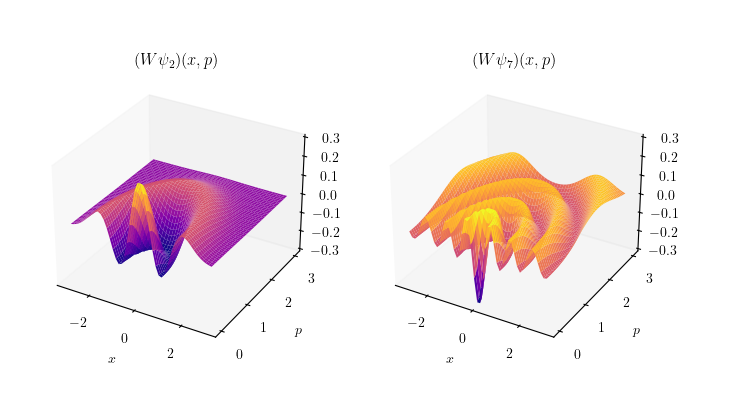
\includegraphics[width=1\textwidth]{
      imgs/harmonic_osc_wigner.png
    }
    \caption{Funciones de Wigner de los estados $\psi_3$ y
    $\psi_7$ del oscilador armónico, con $\hbar = 1$ y
    $\omega = 1$.}
    \label{fig:harmonic_osc_wigner_3_7}
  \end{figure}

  \subsection{Propiedad básica de tomografía cuántica}

  Wootters [CITE1987] expone una propiedad fundamental de la
  función de Wigner, la que el llama la propiedad
  proyectiva. Si $W_\rho$ es la función de Wigner de un
  estado $\rho$, entonces podemos considerar la integral de
  $W_\rho$ sobre una franja infinita delimitada por dos
  rectas paralelas $ax+bp=c_1$ y $ax+bp=c_2$. Resulta que la
  integral es igual a la probabilidad de que se observebe un
  valor entre $c_1$ y $c_2$ del observable
  $a \hat X + b \hat P$.  Integrando sobre una sola recta
  brinda la densidad marginal del operador correspondiente.
  Ésto es una generalización de las  densidades de posición
  y de momentum y se ha demostrado que sí se exige ésta
  propiedad a una cuasi-distibución del espacio de fase, la
  función de Wigner se vuelve única [CITE]. Si tenemos un
  conjunto completo de éstas ``marginales generalizadas'',
  podemos recuperar la distribución conjunta sobre todo el
  espacio. Braasch et al. [Braasch] le llama a éste conjunto
  de marginales un conjunto tomograficamente completo. La
  función de Wigner discreta que definen Wootters
  será basada principalmente en ésta propiedad, en donde en
  lugar de integrar sobre franjas infinitas se suma sobre
  rectas en el espacio de fase discreto.

  \chapter{Funciones de Wigner en el Espacio Fase Discreto}

  Resumiendo el capítulo anterior, podemos representar a un
  estado cuántico por medio de la transformación de Wigner.
  A pesar de no ser una densidad probabilística verdadera
  sobre el espacio de fase, comparte varias propiedades, en
  particular nos permite calcular los valores esperados de
  observables cuánticos y nos permite recuperar las
  densidades probabilísticas de la posición y del momentum
  integrando la función de Wigner sobre el eje de momentum o
  de posición respectivamente. Ésta última característica
  solamente es un caso partícular de una propiedad más
  general de la función de Wigner, la cual es muy útil para
  la tomografía cuántica y que de hecho la vuelva única
  entre las cuasi-distribuciones alternativas.

  Durante las últimas decadas han existido múltiples
  intentos de generalizar la función de Wigner a sistemas
  cuánticos de dimensión finita. Parte fundamental de ésta
  generalización es la definición adecuada del espacio de
  fase discreto. Para un sistema de dimensión $d$, la
  mayoría de construcciones emplean una malla de tamaño $d
  \times d$ e intentan definir una función de Wigner
  evaluada en cada par $\alpha$ de la malla. Como menciona
  Gross [THESIS], parece que existen dos caminos claros en
  la construcción de la versión discreta: un camino intenta
  definir la función de Wigner discreta de una manera
  análoga a la versión continua, i.e., identificando el
  espacio de fase discreto con las variables de posición y
  de momentum, construyendo los operadores de desplazamiento
  y luego los puntuales, para luego definir la función
  utilizando la expresión (). La ventaja de éste camino es
  que la definición discreta asemeja lo más posible al caso
  continuo y sus a interpretaciones.  Ésta versión se puede
  encontrar en los trabajos de Klimov, Sanches y Soto
  [CITE], Paz [CITE], Vourdas [CITE], Gross [CITE], etc. El
  segundo camino dominante es el que intenta definir la
  función discreta a partir de la preservación de las
  propiedades más importantes del caso continuo, en
  particular la propiedad tomográfica. Ésta versión se debe
  a Wootters [CITE] y la idea es identificar una
  \textit{estructura cuántica} al espacio de fase discreto,
  la cual permite que la función de Wigner exprese las
  mismas propiedades que la versión discreta.  Los
  operadores de desplazamiento y los puntuales vuelven a
  aparecer, pero se introduce un tipo de arbitrariedad y de
  flexbilidad, perdiendo la unicidad pero permitiendo una
  construcción alternativa. Además ésta segunda metodología
  expone una relación directa con la construcción de bases
  mutuamente insesgadas.

  Se sabe que el número máximo de bases mutuamente
  insesgados para un sistema cuántico de dimensión $d$ es
  $d+1$, y en particular si la dimensión es una potencia de
  un número primo, entonces siempre se puede alcanzar la
  cantidad máxima [CITE]. Parece que aun es un problema
  abierto identificar la cantidad máxima para dimensiones
  que no son potencias de números primos. La construcción de
  Wootters requiere de la construcción explícita
  de las $d+1$ MUBs para la definición de los operadores
  puntuales y como consecuencia la definición de la función
  de Wigner. Ésto es una consecuencia natural de
  exigir que la función discreta satisfaga las mismas
  propiedades tomográficas que satisface la versión
  continua. Por éstas razones nuestro trabajo se basa en la
  metodología de Wootters.
  %\section{Construcción análoga}

  %Tal como en el caso continuo, existe un mapeo del espacio
  %de Hilbert al espacio de fase que se puede interpretar
  %como una cuasi-distribución conjunta sobre dos variables
  %`conjugadas'. Schwinger desarrolló una base ortonormal de
  %$N^2$ operadores unitarios que forman una representación
  %del grupo de Heisenberg-Weyl modulo su centro. Dado la
  %base ortonormal de operadores, se puede describir al
  %estado de un sistema utilizando los coeficientes de la
  %expansión del operador de densidad en términos de la base.
  %El trabajo consiste en elegir a la ``mejor'' base que
  %resulte en las propiedades de la función de Wigner que
  %deseamos preservar.  La idea de Wooters es construir una
  %versión discreta de los operadores puntuales que preservan
  %las propiedades. 

  %Empezando con la transformada de Fourier discreta y
  %restringiendonos a dimensiones primas impares, podremos
  %trabajar en analogía al caso continuo. El grupo de
  %desplazamientos de Heisenberg-Weyl nos darán los
  %operadores de paridad desplazados, los cuales se usarán
  %para asignar puntos del espacio de fase a operadores.

  %Un sistema cuántico con una espacio de Hilbert de
  %dimensión $N$ será representado por un arreglo de $N
  %\times N$ puntos. Los puntos $\alpha$ estarán dados por
  %los pares $(a_1,a_2)$ de elementos de un campo finito
  %$\Z_n$.

  %Existe una base ortonormal de $N$ elementos para nuestro
  %espacio de Hilbert, correspondientes a los eigenestados de
  %algún observable. Denominemos a éste observable como la
  %``posición'' y diagramaticamente denotará el eje
  %horizontal. Sus eigenvalores denotarán la coordenada del
  %eje horizontal. Lo que sigue es identificar las lineas
  %perpendiculares al eje horizontal del espacio de fase con
  %los eigenestados que corresponden a los eigenvalores. El
  %eje vertical será la variable Fourier-conjugada de la
  %posición llamada el ``momentum''.

  \section{Construcción de Wootters}

  En su artículo del 2004 [CITE], Wootters comienzan notando
  que la función de Wigner en sistemas continuos puede ser
  obtenida al exigir una estructura cuántica al espacio de
  fase. Ésta estructura corresponde a la asignación de
  estados cuánticos a rectas en el espacio de fase, de tal
  manera que las integrales sobre éstas rectas o franjas de
  rectas nos dan la probabilidad de observar el sistema en
  el estado correspondiente, tal como se mencionó en la
  sección anterior. Con ésta asignación, es posible
  recuperar los operadores puntuales y así construir la
  función de Wigner para un estado arbitrario $\rho$.
  Wootters intentan definir una versión discreta siguiendo
  éstos pasos, cuidando que la construcción preserve otras
  propiedades de la versión continua.  Resulta que su método
  introduce cierto tipo de arbitrariedad por lo que acaban
  definiendo una clase de funciones discretas.

  Evidentemente hay una relación directa entre la geometría
  del espacio de fase y la estructura cuántica por asignar.
  Por lo tanto requerimos trabajar con un espacio de fase
  que tenga la suficiente estructura geométrica como para
  definir rectas en el espacio con las propiedades usuales
  que conocemos del plano Euclideano.  Por ejemplo debemos
  poder definir rectas paralelas y se debe cumplir que dos
  rectas no paralelas solo se intersecten en un solo punto.
  Si $d$ es la dimensión del espacio de Hilbert en cuestión,
  es natural intentar definir el espacio de fase como la
  malla $\Z_d \times \Z_d$. Pero si $d$ no es un número
  primo, $\Z_d$ solo es un anillo y resulta que el espacio
  $\Z_d \times \Z_d$ no tiene la estructura geométrica
  necesaria, por ejemplo no es dificil encontrar ejemplos de
  rectas no paralelas que se intersectan en más de un solo
  punto. En el caso en que $d = p$ es un número primo, la
  estructura algebráica $\Z_p$ es un campo y aquí sí se
  puede definir un espacio de fase $\Z_p \times \Z_p$ con
  las propiedades deseadas.  Además de los campos $\Z_p$,
  también podemos obtener campos de orden $p^{n}$ donde $p$
  es primo, por medio de la extension de Galois $\GF(p,n)$.
  La restricción a espacios de Hilbert dimensión $p^{n}$ sí
  es limitante, pero Wootters hacen la observación que su
  método es válido para el importante caso de un sistema de
  $n$ qubits. Por lo tanto su metodología es directamente
  aplicable a los modelos de la computación e información
  cuántica.

  El método consiste en darle una estructura cuántica al
  espacio de fase $\GF(p,n) \times \GF(p,n)$ asignando un
  estado cuántico a cada linea del espacio de fase discreto.
  Ésta asignación debe satisfacer varias propiedades y
  Wootters llaman aquellas asignaciones adecuadas,
  \textit{`redes cuánticas'}. Cada red cuántica define una
  versión de la función de Wigner, pero es posible hacer una
  clasificación en clases de equivalencia para reducir un
  poco la arbitrariedad. La asignación particular de estados
  cuánticos a las rectas de conjuntos de rectas paralelas
  resultan ser bases ortonormales del espacio de Hilbert y
  además son mutuamente insesgadas respecto a otros
  conjuntos de rectas paralelas.

  Para comenzar, recordemos las propiedades de la función de
  Wigner $W_\rho$ del caso continuo que se desean
  perservar en el caso discreto:
  \begin{proposition}
    Sea $\rho$ un operador de densidad y $W_\rho$ su función
    de Wigner.
    \begin{enumerate}
      \item $W_\rho$ es covariante bajo traslaciones.
      \item Los operadores puntuales forman una base
        ortonormal respecto al producto interno de
        Hilbert-Schmidt para el espacio de operadores sobre
        $\H$.
      \item $W_\rho$ es real y la suma de sus componentes
        debe ser igual a $1$.
      \item La integral de $W_\rho$ sobre una
        recta $ax+bp = c$ nos brinda la probabilidad de
        medir el valor $c$ del operador $a \hat X + b \hat P$.
    \end{enumerate}
  \end{proposition}
  
  Recordemos que éstas propiedades pueden ser demostradas a
  partir de las propiedades análogas de los operadores
  puntuales. En particular para la propiedad (4), si $ax+bp
  = c$ es un recta en el espacio de fase, entonces
  integrando (formalmente) a los operadores puntuales sobre
  ésta recta nos da una proyección ortogonal
  $\Pi_{\ket{abc}}$ donde $\ket{abc}$ es un eigenestado del
  operador $a\hat X + b\hat P$ correspondiente al eigenvalor
  $c$ [CITE]. Ésta es parte fundamental para la definición
  de la función discreta, mientras que la propiedad de ser
  covariante bajo traslaciones es la que define a los
  operadores de desplazamiento discretos en la metodología
  de Wootters. 
    
  \subsection{La geometría del espacio de fase discreto}

  El espacio de fase discreto será un espacio vectorial de
  dos dimensiones sobre un campo finito, donde los puntos
  serán etiquetados con los elementos $(x,p) \in
  \mathbb F_{d} \times \mathbb F_{d} = \mathbb F_d^{2}$. Por
  convención, consideramos el punto $(0,0)$ como el origen
  de nuestra malla de $d \times d$ elementos, ubicado en la
  parte inferior izquierda. La construcción de Wootters y
  Gibbons permite identificar el horizontal con los
  eigenvectores de una clase de operadores y el eje vertical
  con otra clase de operadores, ésto a su vez nos permite
  darle cierta interpretación física, aunque ésto no es
  necesario. Por ejemplo si consideramos un sistema cuántico
  de dos partículas con spin-$\frac{1}{2}$, entonces el
  espacio de Hilbert correspondiente es $\H = \C^{2} \otimes
  \C^{2}$, y el espacio de fase discreto sería una malla de
  $4 \times 4$ elementos. Los elementos de la malla serán
  indexados por los elementos de un campo finito de cuatro
  elementos:
  \[
    \mathbb F_4
    = \GF(2,2)
    = \{0,1,\omega,\omega+1\}.
  \]
  En caso de un sistema que no es compuesto, por ejemplo una
  partícula de tres niveles, $\H = \C^3$, el espacio de fase
  discreto es una malla de $3 \times 3$ en donde los
  elementos de la mallan son indexados simplemente con los
  enteros $\Z_3 = \{0,1,2\}$. La figura
  (\ref{fig:GF22-GF31}) muestra el espacio de fase de éstos
  dos ejemplos, y se muestra la linea recta parametrizada
  por $\lambda = \{(s,s) : s \in \mathbb F_d\}$.
  \begin{figure}
    \centering
    \subfloat[\centering $\mathbb F_4 = \GF(2,2)$]{{
        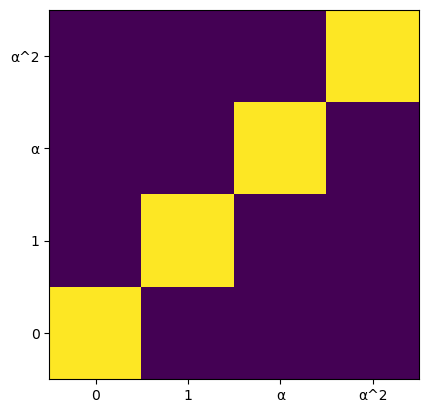
\includegraphics[width=0.4\linewidth]{imgs/GF22.png}
    }}
    \quad
    \subfloat[\centering $\mathbb F_3 = \Z_3$]{{
        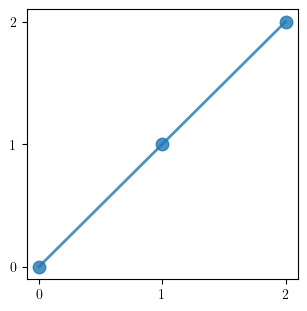
\includegraphics[width=0.38\linewidth]{imgs/GF31.png}
    }}
    \caption{Dos espacios de fase discretos para sistemas de
    distinta dimensión, señalando el rayo diagonal.}
    \label{fig:GF22-GF31}
  \end{figure}
  Como se mencionó antes, una \textit{recta} en el espacio
  de fase es el conjunto de puntos que satisfacen la
  ecuación $ax + bp = c$ donde $a,b$ y $c$ son elementos del
  campo finito. Dos rectas paralelas son iguales si solo
  difieren en el valor de $c$.  No es dificil probar que
  dada una recta $\lambda$ y un punto $\alpha$ que no
  pertenece a la recta existe una única recta paralela a
  $\lambda$ que contiene a $\alpha$.  Similarmente, dos
  rectas que no son paralelas solo se intersectan en un solo
  punto. Existen $N(N+1)$ rectas en el espacio de fase y el
  conjunto de éstas rectas se particiona en $N+1$ conjuntos
  de $N$ rectas paralelas. A cada conjunto de $N$ rectas
  paralelas, se le conoce como un estría. 

  Para ejemplifcar la estrías completas de un espacio de
  fase discreto, consideremos un campo finito de ocho
  elementos. En éste caso el espacio de fase es el espacio
  vectorial $\mathbb F_8^2$ donde $\mathbb F_8$ es una
  extensión de Galois del campo primo $\Z_2$ de grado $n =
  3$, i.e., $\mathbb F_8 = GF(2,3)$.  De acuerdo al apéndice
  (), para construir a $\mathbb F_8$ solo debemos elegir un
  polinomio irreducible $f(x)$ con coeficientes en $\Z_2$ de
  grado $n = 3$ y adjuntarle una raíz $\alpha$ del polinomio
  al campo primo. Así
  \[
    \mathbb F_8
    = \mathbb Z_2(\omega)
    \cong \mathbb Z_2[x] / \langle f(x) \rangle.
  \] 
  Sea $f(x) = x^3+x^2+1$ tal polinomio irreducible y
  $\omega$ una raíz primitiva. Entonces el campo de Galois
  $\mathbb F_8$ está dado por el conjunto 
  \[
    \{0,1,\omega,\omega^2,\omega^2+1,\omega^2+\omega+1,
    \omega+1,\omega^2+\omega\},
  \] 
  con sus correspondientes operaciones de suma y
  mutliplicación. Las rectas verticales estarán dadas por
  los conjuntos $\{(q,s) : s \in \mathbb F_8\}$ donde
  fijamos el elemento $q$ para cada recta vertical. El resto
  de las rectas pueden ser parametrizadas como $\{(q,mq+c) :
  m, c \in \mathbb F_8\}$. La figura (\ref{fig:GF-2-3})
  muestra todas las estrías de éste espacio de fase.

  \begin{figure}[ht]
    \centering
    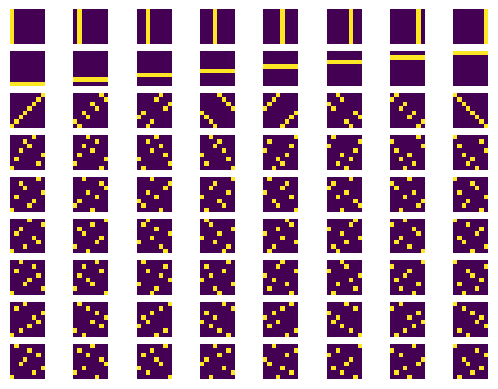
\includegraphics[width=0.7\textwidth]{imgs/GF23.png}
    \caption{Las nueves estrías del espacio de fase $\mathbb
    F_8^2 = \GF(2,3) \times \GF(2,3)$.}
    \label{fig:GF-2-3}
  \end{figure}

  Otro aspecto importante inicial en la metodología de
  Wootters es la noción de las traslaciones en el
  espacio de fase. En el caso discreto no existen
  traslaciones infinitesimales, pero podemos definir una
  traslación como la suma de un vector a los puntos del
  espacio de fase. Si $\alpha \in \mathbb F_d^2$, entonces
  la traslación $\mathcal T_\alpha$ se define simplemente
  como
  \begin{equation}
    \mathcal T_\alpha \beta = \alpha + \beta,
    \quad
    \text{para todo } \beta \in \mathbb F_d^2.
  \end{equation} 

  \subsection{Asignación de la estructura cuántica}

  Para vincular el sistema cuántico con nuestro espacio de
  fase discreto, la clave del método Wootters y Gibbons es
  asignar un estado cuántico a cada una de las $d(d+1)$
  lineas rectas del espacio de fase. De aquí en adelante
  consideramos un sistema cuántico con espacio de Hilbert de
  dimensión $d = p^{n}$ donde $p$ es un número primo. Éste
  método es aplicable de manera natural a sistemas
  compuestos de $n$ subsistemas de dimensión $p$:
  \begin{equation}
    \H^{\otimes n}
    = \H \otimes \cdots \otimes \H,
    \quad
    \text{donde } \dim\H = p.
  \end{equation}
  Un mapeo $Q$ que asigna
  una proyección ortogonal correspondiente a un estado puro
  $Q(\lambda)$ a cada recta $\lambda$ que satisface ciertas
  propiedades deseables se llamará red
  cuántica. La primera propiedad que debe satisfacer la red
  cuántica es la propiedad de ser covariante bajo
  traslaciones, para ésto, debemos definir una versión
  discreta de los operadores de Heisenberg-Weyl $ D(x,p)$
  para cada $(x,p) \in \mathbb F_d^2$. De ésta
  manera a cada traslación en el espacio de fase discreto le
  corresponderá un operador unitario en el espacio de
  Hilbert. Éstos operadores deben tener una regla de
  composición que preserve de algún modo la composición de
  traslaciones en el espacio de fase. Para lograr ésto,
  primero hay que considerar dos operadores básicos,
  correspondientes a traslaciones horizontales y verticales
  de una unidad, las cuales actúan sobre los subsistemas
  cuánticos individuales.

  A la traslación horizontal del espacio de fase $\mathcal
  T_{(1,0)}$ y la traslación vertical $\mathcal T_{(0,1)}$
  les asociamos los operadores unitarios $X$ y $Z$ definidos
  de la siguiente manera:
  \begin{definition}
    Sea $\{\ket k : k \in \Z_p\}$ una base ortonormal del
    espacio de Hilbert $\mathcal H$ correspondiente a un
    subsistema, cuyos vectores se etiquetan con los elementos
    del campo primo. Definimos los siguientes operadores:
    \begin{align}
      X \ket k
      &= \ket{k + 1}, \\
      Z \ket k
      &= \omega^{k} \ket k,
    \end{align}
    donde $\omega = e^{2\pi i / p}$ y donde la suma dentro
    de los kets se hace módulo $p$, i.e., la suma es la del
    campo finito $\Z_p$.
  \end{definition}
  El uso de los números del campo primo como etiquetas
  implica una estructura cíclica a las potencias del
  operador $X$ y comunmente se le dice el operador
  \textit{shift} porque en el caso continuo representan
  cambios en la posición. Similarmente el operador $Z$ se le
  conoce como el operador \textit{boost} porque en el caso
  continuo representa un empuje en términos del momentum.
  Éstos operadores son generadores del grupo de Pauli y
  satisfacen las siguientes propiedades importantes:
  \begin{equation}
    X^{p} = Z^{p} = 1,
    \quad
    X^{a} Z^{b} = \omega^{-ab} Z^{b} X^{a},
    \quad
    \Tr(X) = \Tr(Z) = 0.
  \end{equation}
  Podemos expresar a éstos operadores en la base
  computacional de la siguiente manera:
  \begin{equation}
    X = \sum_{k \in \Z_p}^{} \ket{k+1}\bra{k}, \\
    \quad
    Z = \sum_{k \in \Z_p}^{} \omega^{k} \ket k \bra k.
  \end{equation}
  \begin{example}
    Para $\H = \C^{2}$ tenemos que $p = 2$ y así las
    matrices $X$ y $Z$ son las matrices de Pauli $\sigma_x$
    y $\sigma_z$:
    \[
      X = \sigma_x
      \begin{pmatrix} 0 & 1 \\ 1 & 0 \end{pmatrix},
      \quad
      Z = \sigma_z
      \begin{pmatrix} 1 & 0 \\ 0 & -1 \end{pmatrix}. 
    \] 
  \end{example}

  Con las definiciones de los operadores generalizados de
  Pauli, pasamos a la cuestión de como definir operadores de
  desplazamiento correspondientes a traslaciones $\mathcal
  T_{(a,b)}$ arbitrarias del espacio de fase. El camino que
  elegin Wootters es construir los operadores a
  partir de productos tensoriales de los elementos del grupo
  de Pauli. De ésta manera se puede lograr actuar sobre los
  subsistemas de manera individual. La asociación del punto
  $(a,b) \in \mathbb F_d^2$ con el operador correspondiente
  del espacio $\H^{\otimes n}$ depende de la expansión de
  $a$ y de $b$ en bases de la extensión de Galois.
  Recordemos que la extensión de Galois $\GF(p,n)$ se puede
  ver como un espacio vectorial de dimensión $n$ sobre el
  campo primo $\Z_p$. Entonces eligiendo una base
  $\{b_1,\ldots,b_n\} \subset \GF(p,n)$ del campo podemos
  expresar a todo elemento $a \in \GF(p,n)$ como la
  combinación lineal:
  \[
    a = \sum_{i=1}^{n} c_i b_i,
    \quad
    \text{donde } c_i \in \Z_p.
  \] 
  De igual manera, debemos elegir una base dual a la base
  del campo finito. Recordemos del apéndice () que una base
  dual es tal que
  \[
    \tr(b_i \tilde b_j) = \delta_{ij},
  \] 
  y que en muchas ocasiones podemos encontrar una base
  \textit{auto-dual}, algo que es conveniente a la hora de
  hacer los cálculos. Dada la base y la base dual, Wootters
  y Gibbons definen a los operadores de desplazamiento
  correspondientes a traslaciones arbitrarias $\mathcal
  T_{(a,b)}$, como productos tensoriales de monomios de los
  operadores unitarios $X$ y $Z$, donde las potencias están
  dadas por los coeficientes de la expansión de $a$ en la
  base y de $b$ en la base dual:
  \begin{definition}
    Sean $a_1,\ldots,a_n$ los coeficientes de $a$ en la base
    del campo y $b_1,\ldots,b_n$ los coeficientes de $b$ en
    la base dual. Entonces definimos al operador de
    desplazamiento como
    \begin{equation}
      D(a,b)
      = X^{a_1} Z^{b_1} \otimes \cdots \otimes X^{a_n}
      Z^{b_n}.
    \end{equation}
  \end{definition}
  Ésta definición parece ser un poco ad-hoc pero es
  inmediato ver que es una correspondencia muy natural con
  las traslaciones básicas del espacio de fase discreto,
  en el sentido de que si una traslación por el vector
  $(a,b)$ solo tiene los $i$-ésimos componentes de $a$ y $b$
  no nulos, entonces el operador de desplazamiento solo
  actúa sobre el $i$-ésimo subsistema.

  El operador $Z$ es diagonal y sus eigenvectores son la
  base estándar de $\C^{p}$, por lo tanto los eigenvectores
  correspondientes a los operadores de desplazamiento de la
  estría vertical, 
  \[
    D(0,b) = Z^{b_1} \otimes \cdots \otimes Z^{b_n},
  \] 
  son los productos tensoriales de la base estándar:
  \[
    \ket{k_1} \otimes \cdots \otimes \ket{k_n},
    \quad k_1,\ldots,k_n \in \Z_p.
  \] 
  Vourdas [CITE] muestra que se puede etiquetar la base
  computacional con elementos de la extensión de Galois
  $\GF(p,n)$ y utilizando una base del campo se pueden
  mapear los elementos de manera natural:
  \[
    \ket \alpha
    \mapsto \ket{\alpha_1} \otimes \cdots \otimes
    \ket{\alpha_n}
  \] 
  donde los $\alpha_1,\ldots,\alpha_n$ son los coeficientes
  de la expansión de $\alpha$. Pero hay un detalle
  importante que surge de la estructura tensorial, Klimov et
  al [CITE] muestran que los estados etiquetados con los
  elementos de la extensión de Galois puede ser mapeados a
  estados fisicos\footnote{Se refieren a los elementos de la
  base computacional y de los vectores abstractos.} con
  \textit{distintas} propiedades de factorización
  dependiendo de la base elegida. Por ésto la elección de la
  base del campo dependerá de la aplicación física.
  \begin{example}
    .
  \end{example}
  Por otro lado, los operadores de desplazamiento respecto a
  las traslaciones horizontales son
  \[
    D(a,0) = X^{a_1} \otimes \cdots \otimes X^{a_n},
  \] 
  y sus eigenvectores están dados por productos tensoriales
  de vectores $\ket{\tilde k}$ donde
  \[
    \ket{\tilde k}
    = \frac{1}{\sqrt{p}} \sum_{k=1}^{p}
    \omega^{\tilde k k} \ket k.
  \] 
  Notemos que ésta última expresión parece una
  transformación de Fourier de la base computacional. De
  hecho Vourdas y otros autores definen una transformación
  de Fourier finita a partir de los caracteres $\chi$ del
  campo finito y construyen una segunda base del espacio de
  Hilbert mediante su aplicación. De ésta manera obtienen
  dos bases `Fourier conjugables' y las asocian con la
  noción de posición (base computacional) y momentum (base
  obtenida por la transformación de Fourier) en el espacio
  de fase discreto. A pesar de ésto Klimov et al. hacen la
  observación que debido a la arbitrariedad de las bases, la
  analogía con la posición y momentum en el espacio de fase
  discreto es un poco forzada [CITEchap7].

  Regresando a la construcción de la función de Wigner,
  utilizando los operadores de desplazamiento podemos
  enunciar el requisito de ser covariante bajo traslaciones
  que le pediremos a la función de Wigner. Dado que la
  función de Wigner dependerá de la red cuántica $Q$,
  conviene que el mapeo $Q$ sea covariante bajo traslaciones
  en el siguiente sentido: si trasladamos una linea por
  $\mathcal T_{(a,b)}$ entonces el estado cuántico también
  debe ser trasladado pero por los operadores de
  desplazamiento correspondientes, i.e.,
  \begin{equation}
    \label{eqn:trans_cov_net}
    Q(\mathcal T_{(a,b)} \lambda)
    = D(a,b) Q(\lambda) D(a,b)^{*}.
  \end{equation}
  Ésto resulta ser un requisito muy fuerte, ya que implica
  que los operadores correspondientes a las traslaciones que
  dejan invariantes a las rectas de una estría deben
  conmutar. Para ver ésto, supongamos que $\lambda$ es un
  rayo parametrizado por $(sx,sy)$ donde $s \in \mathbb
  F_d$. Entonces ésta recta y todas las rectas paralelas a
  ella son invariantes bajo las traslaciones $\mathcal
  T_{(tx,ty)}$ donde $t \in \mathbb F_d$:
  \begin{align*}
    \mathcal T_{(tx,ty)} \lambda
    &= \{(tx,ty) + (sx,sy) : (sx,sy) \in \lambda \} \\
    &= \{((t+s)x, (t+s)y) : t+s \in \mathbb F_d \}\\
    &= \lambda.
  \end{align*} 
  La ecuación (\ref{eqn:trans_cov_net}) nos dice entonces
  que
  \[
    D(tx,ty) Q(\lambda) D(tx,ty)^{*}
    = Q(\mathcal T_{(tx,ty)}\lambda)
    = Q(\lambda),
  \] 
  lo cual solo sucede si los operadores de desplazamiento
  conmutan con $Q(\lambda)$ para cada $t \in \mathbb F_d$.
  Ésto a su vez solo sucede si los operadores de
  desplazamiento $D(tx,ty)$ para $(x,y)$ fijo conmutan entre
  si. En otras palabras, para que la red cuántica sea
  covariante bajo traslaciones, los operadores de
  desplazamiento correspondientes a las traslaciones que
  dejan una estría invariante deben conmutar (PROOF).
  Gibbons y Wootters prueban que su definición de $D(a,b)$
  satisface éste requisito si y solo si la base en que se
  expande el vector $b$ es un \textit{múltiplo} de la base
  dual. Ésto introduce otro punto de arbitrariedad que a
  nosotros nos gustaría evitar, por lo tanto en general
  simplemente tomamos la base dual como la segunda base,
  eligiendo la auto-dual cuando ésta exista.

  Los operadores de desplazamiento así construidos son de
  traza nula y son mutuamente ortogonales respecto al
  producto interno de Hilbert-Schmidt:
  \[
    \Tr\left( \hat D(sx,sy) \hat D(tx,ty)^{*} \right) 
    = 0,
    \quad s \neq t.
  \] 
  Por lo tanto definen una única base de eigenvectores
  simultáneos (salvo fases globales). Aquí surge la
  propiedad más atractiva de la construcción de Wootters y
  Gibbons que depende de un resultado de Bandyophyay et al
  [CITE]:
  \begin{theorem}[Bandyophyay et al. Thereom 3.2]
    Si existe una base conmutativa maximal de matrices
    unitarias ortogonales, entonces existen un conjunto de
    $d+1$ bases mutuamente insesgadas.
  \end{theorem}
  En éste caso una \textit{base conmutativa maximal} de
  matrices unitarias ortogonales se refiere a una partición
  de matrices unitarias ortogonales en $N+1$ conjuntos donde
  las $N-1$ matrices de cada clase conmutan entre si.
  Notemos que la agrupación de los operadores invariantes de
  cada estría satisface ésta condición, por lo que Wootters
  y Gibbons concluyen que los conjuntos de eigenvectores
  simultáneaos forman un conjunto de bases mutuamente
  insesgadas. Regresando un poco al tema de Klimov et al.,
  notemos que el uso de distintas base del campo finito
  implica que podemos obtener bases mutuamente insesgadas
  con distintas propiedades de factorización.

  Hasta ahorita solo se ha asignado una base ortonormal a
  cada estría. Para construir el mapeo $Q$ debemos
  identificar a cada linea de cada estría con un elemento de
  la base. Resulta que podemos asignar un elemento de la
  base al rayo $\lambda$ de la estría de manera
  \textit{arbitraria}.  El resto de la asignación se
  determina por los mismos operadores de desplazamiento:
  \[
    Q(\mathcal T_{(x,y)} \lambda)
    = D(x,y) Q(\lambda) D(x,y)^{*},
  \] 
  ya que se pueden obtener el resto de las rectas de la
  estría mediante traslaciones en el espacio de fase.  Las
  elecciones arbitrarias hasta el momento dan distintas
  definiciones de las redes cuánticas y como consecuencia
  distintas funciones de Wigner, cuya definición obtenemos
  enseguida.

  \subsection{Definición de una función de Wigner}

  Sea $\rho$ un operador de densidad y $W_\rho$ su función
  de Wigner por definir. Para preservar la propiedad
  tomográfica básica de la función de Wigner en el caso
  discreto, requerimos que la suma de $W_\rho$ sobre la
  recta $\lambda$, sea la probabilidad de que el sistema
  cuántico se mida en el estado $Q(\lambda)$. Ésto significa
  que 
  \begin{equation}
    \label{eqn:tomog_prop_discrete}
    \sum_{\alpha \in \lambda}^{} W_\rho(\alpha)
    = \Tr\left( \rho Q(\lambda) \right).
  \end{equation}
  Dado que nuestro espacio de fase es una geometría finita,
  a traves del punto $\alpha$ pasan exactamente $d+1$
  rectas que cubren a todo el espacio de fase discreto.
  Entonces si $W_\rho$ satisface la propiedad de
  normalización, i.e., $\sum_\beta W_\rho(\beta) = 1$, se
  cumple que
  \begin{equation}
    \sum_{\lambda \ni \alpha}^{}
    \left( \sum_{\beta \in \lambda}^{} W_\rho(\beta) \right) 
    = d W_\rho(\alpha) + 1.
  \end{equation}
  Despejando obtenemos un expresión para $W_\rho(\alpha)$:
  \[
    W_\rho(\alpha)
    = \frac{1}{d}
    \left[
      \sum_{\lambda \ni \alpha}^{}
      \left(
        \sum_{\beta \in \lambda}^{} W_\rho(\beta)
      \right) - 1,
    \right]
  \] 
  y utilizando (\ref{eqn:tomog_prop_discrete}) tenemos
  \begin{equation}
    W_\rho(\alpha)
    = \frac{1}{N} \left( \sum_{\lambda \ni \alpha}^{}
    \Tr\left( \rho Q(\lambda) \right) - 1 \right).
  \end{equation}
  Utilizando las propiedades de la traza podemos expresar
  la función de Wigner en términos del valor esperado de un
  operador $A(\alpha)$ en estado $\rho$:
  \begin{equation}
    \label{eqn:discrete_wigner}
    W_\rho(\alpha)
    = \frac{1}{N} \Tr\left( \rho A(\alpha) \right),
  \end{equation} 
  donde 
  \begin{equation}
    \label{eqn:discrete_point_op}
    A(\alpha)
    = \sum_{\lambda \ni \alpha}^{} Q(\lambda) - I.
  \end{equation} 
  Los operadores $A(\alpha)$ son los ánologos a los
  operadores puntuales $\hat \Delta(\alpha)$ en el caso
  continuo, por lo que también lleverán el mismo nombre.

  Por construcción la función de Wigner discreta
  satisface la propiedad tomográfica básica y la propiedad
  de normalización. Probando ciertas propiedades de los
  operadores puntuales $A(\alpha)$ análogos a las
  propiedades los operadores $\hat \Delta(\alpha)$, podremos
  probar las otras propiedades deseables de la función de
  Wigner.
  \begin{proposition}
    Los operadores puntuales $A(\alpha)$ donde $\alpha =
    (a,b) \in \mathbb F_d^2$ satisfacen las siguientes
    propiedades:
    \begin{itemize}
      \item $A(\alpha)$ es auto-adjunto.
      \item Son de traza unitaria.
      \item Son ortogonales bajo el producto interno de
        Hilbert-Schmidt.
    \end{itemize}
  \end{proposition}
  \begin{proof}
    .
  \end{proof}

  En particular notemos que los operadores $A(\alpha)$ 
  forman una base del espacio de operadores lineales del
  espacio de Hilbert. Así que podemos expresar a cualquier
  operador de densidad en términos de los operadres
  puntuales
  \[
    \rho = \sum_{\alpha}^{} a_\alpha A(\alpha).
  \] 
  Utilizando la propiedad (3) de los operadores puntuales
  podemos probar que los coeficientes en la expansión son
  precisamente los valores de la función de Wigner en el
  punto $\alpha$:
  \[
    \rho = \sum_{\alpha}^{} W(\alpha) A(\alpha).
  \] 
  Con ésto tenemos una representación completa de cualquier
  estado cuántico en el espacio de fase discreto, y a partir
  de una función de Wigner podemos recuperar el estado
  correspondiente mediante la expansión en los operadores
  puntuales. Concluímos ésta sección enlistando las
  propiedades que hereda la función de Wigner de los
  operadores puntuales:
  \begin{proposition}
    Sea $\rho$ un estado cuántico y $W_\rho$ su función de
    Wigner discreta. Entonces
    \begin{enumerate}
      \item La función de Wigner es real.
      \item La suma de $W_\rho$ sobre cualquier recta
        $\lambda$ es igual al valor esperado de $Q(\lambda)$ 
        en el estado $\rho$.
      \item La suma de $W_\rho$ sobre todo el espacio de fase
        es igual a 1.
      \item La función de Wigner es covariante bajo
        traslaciones.
    \end{enumerate}
  \end{proposition}
  \begin{proof}
    .
  \end{proof}

  \section{Ejemplos}

  \chapter{Construcción no-estándar}

  La elección de asignar elementos de bases mutuamente
  insesgadas a rectas en el espacio de fase es lo
  que distingue la construcción de Wootters de otros métodos
  de construcción de funciones de Wigner. Como hemos visto
  la idea reside en particionar el espacio de fase discreto
  en \textit{rectas} paralelas, pero resulta que ésta no es la
  única manera de particionar una malla de $d \times d$ 
  en conjuntos de puntos tales que cualesquiera dos puntos
  distintos residen en uno solo de esos conjuntos. Éstos
  objetos han sido estudiados en otras áreas de las
  matemáticas, por ejemplo en la combinatoria y donde
  llevan el nombre de planos afínes. 

  \begin{definition}[Plano afín]
    Un plano afín de orden $d$ es un objeto combinatorio que
    consiste de un conjunto de $d^2$ puntos, junto con
    $d(d+1)$ conjuntos de puntos llamados \textit{lineas},
    tales que cualesquiera dos puntos distintos pasa por una
    única linea. En éste caso las lineas se pueden agrupar
    en $d+1$ clases de lineas `paralelas' de tamaño $d$,
    particionando a todo el conjunto de puntos. 
  \end{definition}

  En su artículo [CITE], Kantor muestra que hay una relación
  íntima entre planos afínes y bases mutuamente insesgadas.
  Ésto lo hace recordando algunos resultados más viejos que
  conectaban planos afínes con otras estructuras algebráicas
  llamadas \textit{spreads simplécticos} y con familias de
  subespacios unidimiensionales mutuamente ortogonales.
  El método de construcción de MUBs de Kantor es lo
  suficientemente general para incluir a las construcciones
  conocidas (incluyendo la de Wootters) y además permite
  construir MUBs que \textit{no} son unitariamente
  equivalente a las construcciones estándares. La idea de
  éste capítulo es utilizar spreads simplécticos (y por ende
  planos afínes) distintos a los de Wootters para obtener
  bases de MUBs no unitariamente equivalentes. Utilizando la
  construcción de Wootters podemos definir una función de
  Wigner que preserve la propiedad tomográfica básica. 

  Así como lo hacen Kantor y Kanat [CITE], por sutilizas de
  los campos finitos de característica par, separamos la
  construcción de MUBs en dos: para espacios de Hilbert de
  dimensión $d = p^{n}$ donde $p$ es par, y en otro cuando
  $p$ es impar.

  \subsection{Característica par}

  Consideremos el espacio de Hilbert $\C^{d}$ con $d =
  2^{n}$. Kantor considera el espacio vectorial $V =
  \Z_2^{n}$ con el producto interno usual $x \cdot y$.
  Denotemos a la base estándar de $\C^{d}$ por $\ket{e_v}$ 
  donde $v \in V$. Kantor define a los generadores del grupo
  de Pauli sobre $\C^{d}$ de la siguiente manera:
  \begin{align}
    X(b) &: \ket{e_v} \mapsto \ket{e_{v+b}} \\
    Z(b) &: \ket{e_v} \mapsto (-1)^{b \cdot v} \ket{e_v},
  \end{align}
  para todo $b \in V$. Utilizando la relación de conmutación
  () del capítulo anterior, Kantor observa que
  \begin{equation}
    (X(a)Z(b))^{-1}(X(a')Z(b'))^{-1} (X(a)Z(b))(X(a')Z(b'))
    = a \cdot b' - a' \cdot b
  \end{equation}
  determina una forma bilineal alternante $(\,,\,)$ sobre el
  espacio $V \oplus V$. Recordemos que una forma bilineal
  sobre un espacio vectorial es una forma alternante si para
  todo $v \in V$, se cumple $(v,v) = 0$.
  \begin{definition}[Kantor]
    Un spread simpléctico de un espacio simpléctico $V
    \oplus V$ es una familia $\Sigma$ de $d+1$ $n$-espacios
    totalmente isotrópicos de $V \oplus V$ tales que su
    intersección uno-a-uno es el espacio trivial $0$. 
  \end{definition}
  Un $n$-espacio totalmente isotrópico es un subespacio de
  dimensión $n$ en donde la forma bilineal se anula. En un
  spread simpléctico, todo vector de $V \oplus V$ está en
  uno y solo un miembro de $\Sigma$, asi que $\Sigma$
  particiona a los vectores no nulos. Kantor nos dice que
  ésto determina un plano afín de orden $d$, cuyos puntos
  son los vectores en $V \oplus V$ y cuyas lineas son
  traslaciones de los miembros de $\Sigma$ por los elementos
  de $V \oplus V$. Por medio spreads simplécticos, Kantor
  relaciona a un plano afín con bases mutuamente insesgadas.

  \begin{theorem}[Kantor (CITE), Teorema 2.3]
    Todo spread simpléctico $\Sigma$ de $V \oplus V$ 
    determina una base completa de $d+1$ MUBs en $\C^{d}$ 
    tales que cada miembro es invariante bajo el grupo de
    Pauli.

    Además, sea $\Sigma'$ es otro spread simpléctico de $V
    \oplus V$, entonces $\Sigma$ y $\Sigma'$ son
    equivalentes bajo una transformación lineal de $V \oplus
    V$ que preserva la forma bilineal alternante si y solo
    si las MUBs respecto a  $\Sigma$ y $\Sigma'$ son
    equivalentes bajo una transformación unitaria de
    $\C^{d}$.
  \end{theorem}

  Resulta que la partición en lineas rectas de Wootters del
  espacio de fase discreto es precisamente un plano afín!
  Por lo tanto el teorema anterior nos dice que si logramos
  encontrar un spread simpléctico no equivalente, (i.e.,
  encontrar un plano afín no isomorfo al de Wootters),
  obtendremos bases mutuamente insesgadas que \textit{no}
  son unitariamente equivalentes. Podremos aplicar el método
  de construcción de Wootters con éstas bases no
  equivalentes para obtener operadores puntuales distintos a
  los de Wootters y por lo tanto una definición
  alternativa de la función de Wigner discreta, que además,
  por construcción, preserva la propiedad tomográfica
  básica. Veamos.

  Consideremos el espacio vectorial de una dimensión $V =
  \GF(2^{n})$ sobre el campo finito $\GF(2^{n})$. Sabemos
  que $V$ también es un espacio vectorial de dimensión $n$ 
  sobre el campo finito $\Z_2$. Definamos la forma bilineal
  alternante
  \[
    \left( (a,b), (c,d) \right) 
    = \tr(ad-bc)
  \] 
  sobre el espacio $V \oplus V = \GF(2^{n})^2$ de dimensión
  $2n$ sobre $\GF(2)$. Entonces el conjunto $\Sigma$ de
  espacios uni-dimensionales sobre $\GF(2^{n})$ de $V \oplus
  V$ es un spread simpléctico de $V \oplus V$ ya que $ad-bc$
  desaparece en cada uno de ellos. Kantor obsserva que
  $\Sigma$ consiste de los subconjuntos
  \[
    x = 0
    \quad \text{ y } \quad
    y = mx,
  \]
  de $V \oplus V = \GF(2^{n})^2$ para $m \in \GF(2^{n})$,
  los cuales reconocemos que son los rayos de las estrías de
  Wootters. Las bases mutuamente insesgadas que se obtienen
  a partir de $\Sigma$ son precisamente las que son
  unitariamente equivalentes a las de Wootters,
  Klappenecker, etc. [CITE]. 

  Kantor menciona que la construcción de spreads
  simplécticos no es fácil pero nos brinda un ejemplo que
  utilizaremos más adelante. Sea $V = \GF(2^{n})$ y
  equipemos a $V \oplus V = \GF(2^{n})^2$ con la misma forma
  bilineal alternante. Entonces asumiendo que $n > 3$ e
  impar, los subconjuntos 
  \[
    x = 0
    \quad \text{ y } \quad
    y = m^2x + m\tr(x) + \tr(mx)
  \]
  de $V \oplus V$ con $m \in V$ es un spread simpléctico de
  $V \oplus V$ que \textbf{no} es equivalente al ejemplo
  anterior. La construcción explícita de las bases es un
  poco latoso debido a que necesitamos \textit{salirnos} del
  campo finito y pasar al anillo de Galois correspondiente.

  Kantor observa que todo spread simpléctico $\Sigma$ en $V
  \oplus V$ consiste de $0 \oplus V$ y $\{(v, Mv) : v \in
  V\}$ para todo $M \in \mathcal K$ donde $\mathcal K$ es el
  conjunto de $|V| = d = 2^{n}$ matrices simétricas de
  tamaño $n \times n$ tales que la diferencia de
  cualesquiera es no singular. Entonces los conjuntos 
  \begin{align}
    \mathcal F_\infty &=
    \{\ket{e_v} : v \in V\}, \\
    \mathcal F_M^{\mathcal K} &=
    \left\{
      \sum_{v \in V}^{} i^{\tr(2 \hat a \cdot \hat v + \hat
      v \cdot \hat M \hat v)} \ket{e_v} : a \in V
    \right\},
  \end{align}
  forman $d + 1$ MUBs. Pero hay un detalle, los `hats'
  simbolizan que las operaciones se hacen en el
  \textit{anillo} $\Z_4$, i.e., $\hat a, \hat v \in \Z_4$.
  El caso $M : x \mapsto mx$ nos brinda las bases de
  Wootters.

  \subsection{Característica impar}

  Ahora consideremos el espacio $\H = \C^{p^{n}}$ donde $p$ 
  es un primo impar. Sea $V = \Z_p^{n}$ con su producto
  interno usual $x \cdot y$. Ahora consideremos la base
  estándar de $\C^{d}$,  $\ket{e_v}$ con $v \in V$. Sea
  $\omega \in \C$ la $p$-ésima raíz primitiva de la unidad.
  Para $b \in V$ de nuevo definimos a los operadores de
  desplazamiento:
  \begin{align}
    X(b) &: \ket{e_v} \mapsto \ket{e_{v+b}} \\
    Z(b) &: \ket{e_v} \mapsto \omega^{b \cdot v}
    \ket{e_v}.
  \end{align}
  El conmutador definido anteriormente de nuevo define una
  forma bilineal alternante sobre $V \oplus V$. En éste caso
  Kantor decide identificar a $\Sigma$ con el conjunto $K$ 
  de $p^{n}$ matrices simétricas $n \times n$ tal que las
  diferencias uno a uno son no-singulares. Así $\Sigma$ 
  consiste de $0 \oplus V$ y todos los conjuntos $\{(v,Mv) :
  v \in V\}$ para $M \in K$. Explícitamente, 
  \[
    \ket{M; a}
    \sum_{v \in V}^{} \omega^{a \cdot v + v \cdot Mv / 2}
    \ket{e_v}, 
    \quad a \in V,
  \] 
  donde $M \in K$, junto con la base estándar es un conjunto
  completo de MUBs para $\C^{p^{n}}$. De nuevo el espacio de
  fase discreto de Wootters es un caso específico de ésta
  construcción, es el caso en que $M : x \mapsto mx$. 


  Kanat de hecho menciona que todas las
  construcciones conocidas de MUBs se habían obtenido a
  partir de algo que se llaman \textit{spreads simplécticos}
  y por \textit{funciones planares} [CITE]. 

  
  Gibbons y Wootters utilizaron los resultados de
  Bandyophyay et al para demostrar que los operadores de
  desplazamiento que corresponden a las traslaciones
  invariantes de una estría son simultáneamente
  diagonalizable. Siguiendo la metodología de Wootters y
  Gibbons sería necesario obtener al menos un eigenvector
  mutuo para cada una de las $d+1$ estrías, algo sería
  computacionalmente latoso conforme la dimensión va
  creciendo. Por suerte existen múltiples construcciones
  explícitas de bases mutuamente insesgadas que son
  unitariamente equivalentes a las de Wootters,
  que podemos utilizar para construir los operadores
  puntuales.

  \section{Construcción explícita de las MUBs}

  Kanat [CITE] menciona que las bases mutuamente insesgadas
  fueron estudiadas por primera vez por Schwinger en 1960,
  pero no fueron definidas y ejemplificadas hasta 1987 por
  parte de Wootters y Fields. Recordemos que un conjunto de
  MUBs en un espacio de Hilbert $\C^{d}$ se define como un
  conjunto de bases ortonormales $\{B_0,B_1,\ldots,B_r\}$ 
  del espacio tales que
  \[
    |\braket{x|y}|^2 = \frac{1}{d},
  \] 
  para cualesquiera dos vectores $x$ y $y$ de bases
  distintas. También comenta que la existencia de un
  conjunto de MUBs completo es equivalente a encontrar una
  descomposición ortogonal del algebra de Lie complejo
  $sl_n(\C)$. Además se ha descubierto que las MUBs están
  intimamente relacionadas con otros problemas en diversas
  áreas de las matemáticas, como el algebra combinatoria y
  la matemática discreta.

  Godsil y Roy [CITE] probaron que las construcciones de
  MUBs más conocidas, debido a Ivánovic [CITE], Wootters y
  Fields [CITE], Klappenecker [CITE] y Bandyophyay [CITE]
  son todos unitariamente equivalentes. En particular
  demuestran que las bases dadas por Wootters y Fields son
  precisamente las que se obtienen de la diagonalización de
  los conjuntos de operadores de desplazamientos que
  conmutan entre sí. Para reproducir las pruebas primero
  definamos a los operadores de desplazamiento de nuevo pero
  ésta vez sin la factorización tensorial. Así el sistema
  cuántico tendrá un espacio de Hilbert de dimensión $d =
  p^{n}$ con $p$ primo. Existen diferencias entre las
  construcciones para $p$ par e impar debido a algunas
  sutilizas de la extensiones de Galois de característica
  dos, por lo tanto igual que Godsil y Roy, separamos los
  dos casos.

  \begin{example}
    3**1 mubs
  \end{example}

  \begin{example}
    2**3 mubs
  \end{example}
  
  ---

  Todas las construcciones de conjuntos completos de MUBs se
  obtuvieron con spreads simpléticos o con funciones
  planares [KANAT]. Sea  $\mathbb F_d$ un campo finito de
  orden $d$. Sea $V$ el espacio vectorial sobre $\mathbb
  F_d$ con su producto escalar usual $u \cdot v$.
  Consideremos el espacio $W = V \oplus V$ como el espacio
  vectorial sobre el campo primo $\Z_p$ y definamos
  la forma bilineal alternante en $W$ como:
  \begin{equation}
    \langle (u,v), (u',v') \rangle
    = \tr\left( u \cdot v' - v \cdot u' \right),
  \end{equation}
  donde de nuevo $\tr : \mathbb F_q \to \Z_p$. Sea $n = |V|$ 
  y sean $\{\ket{e_w}\}$ la base estándar de $\C^{n}$ 
  indexada por los elementos de $V$. Sea $\omega \in \C$ la
  $p$-ésima raíz primitiva de la unidad. Para todo $u \in V$ 
  definamos a las martices de Pauli generalizadas de la
  siguiente manera:
  \begin{align}
    X(u) &: \ket{e_w} \mapsto \ket{e_{w+u}} \\
    Z(v) &: \ket{e_w} \mapsto \omega^{\tr(v \cdot w)}
    \ket{e_w}.
  \end{align}
  Las matrices $D(u,v) = X(u)Z(v)$ forman una base del
  espacio de matrices complejas de tamaño $n \times n$. Más
  aún, las matrices $D(u,v)$ (con $(u,v) \neq (0,0)$),
  generan al algebra de Lie compleja $sl_n(\C)$. Recordando
  la relación de conmutación de las matrices de Pauli,
  podemos probar que el conmutador de dos operadores
  $D(u,v)$ y $D(u',v')$ es
  \begin{equation}
    [D(u,v), D(u',v')]
    = \omega^{\tr(v \cdot u')}
    \left( 1 - \omega^{\langle (u,v), (u',v') \rangle}
    \right) D(u+u',v+v').
  \end{equation}
  Por lo tanto dos operadores de desplazamiento conmutan si
  y solo si $\langle (u,v), (u',v') \rangle = 0$.

  Ahora consideremos a $V$ el espacio vectorial de dimensión
  $r$ sobre $\mathbb Z_p$. Kanat define a un spread
  simpléctico del espacio simpléctico $2r$-dimensional $W =
  V \oplus V$ sobre $\Z_p$ como una familia de $n+1$ 
  subespacios de dimensión $r$ totalemente isotrópicos de
  $W$ tales que que cada punto de $W$ no 0 reside en un
  único subespacio. Sea
  \[
    \Sigma = W_0 \oplus W_1 \oplus \cdots \oplus W_n,
  \] 
  entonces existe una descomposición ortogonal  del algebra
  de Lie $sl_n(\C)$ dado por:
  \begin{equation}
    L = H_0 \oplus H_1 \oplus \cdots \oplus H_n,
    \quad
    H_i = \langle D(u,v) | (u,v) \in W_i \rangle.
  \end{equation}

  \subsection{Kanat: Spreads simplécticos en característica
  impar}

  Ahora Kanat nos demuestra como construir un conjunto
  completo de MUBs a partir del spread symplectico
  utilizando semi-campos. Sea $\mathbb F_q$ un campo finito
  de orden $q = p^{r}$ con $p$ un primo impar.
  \begin{definition}
    Un subespacio totalmente isotrópico es un subespacio
    vectorial de un espacio con producto interno sobre el
    cual la forma bilineal se anula.
  \end{definition}
  Kanat muestra que si $\Sigma$ es un spread simpléctico de
  $W = V \oplus V$ y dado un $h : V \to V$ tal que
  \[
    \{(u,h(v)) : u \in V\}
  \] 
  es un subespacio totalmente isotrópico maximal, entonces
  \[
    \tr(u \cdot h(w))
    = \tr(h(u) \cdot w)
  \] 
  para todo $u,w \in V$. Con ésto Kanat demuestra la
  siguiente proposición.
  \begin{proposition}
    Sea $\Sigma$ un spread simpléctico de $W = V \oplus V$,
    y sea $h : V \to V$ un mapeo lineal tal que $\{(u,h(u))
    : u \in V\}$ es un subespacio totalmente isotrópico
    maximal. Entonces para todo $v \in V$, el vector
    \[
      \ket{b_{h,v}}
      = \sum_{w \in V}^{} \omega^{\tr\left( \frac{1}{2} w
      \cdot h(w) + v \cdot w \right) } \ket{e_w},
    \] 
    es un eigenvector del operador $D(u,h(u))$ para todo $u
    \in V$.
  \end{proposition}
  Ésta proposición nos permite constuir un conjunto completo
  de MUBs que corresponden a una descomposición ortogonal
  del algebra de Lie $sl_n(\C)$ que a su vez se obtuvo de un
  spread sympléctico. ¿Cómo construir spreads simplécticos?
  Kanat propone utilizar semicampos. Un presemicampo finito es
  un anillo sin divisores de cero, y que satisface la
  distributividad. Un presemicampo finito con una identidad
  multiplicativa es un semicampo. Siempre podemos obtener un
  presemicampo a partir de un campo finito al introducir un
  operación nueva $*$. Todo presemicampo determina un spread
  $\Sigma$ que consiste de subespacios $(0,\mathbb F_d)$ y
  $\{(x, x * y) : x \in \mathbb F_d\}$ para $y \in \mathbb
  F_d$. Un presemicampo es simpléctico si su spread
  simpléctico correspondiente es simpléctico respecto a
  algúna forma bilineal alternante.

  \begin{theorem}[Kanat (CITE) Teorema 3.3]
    Sea $(\mathbb F_d, +, \circ)$ un presemicampo
    simpléctico finito de característica impar. La base
    estándar indexado por los elementos del campo finito y
    las bases $B_m = \{\ket{b_{m,v}} : v \in \mathbb F_d\}$ 
    con $m \in \mathbb F_q$ dados por
    \[
      \ket{b_{m,v}}
      = \frac{1}{\sqrt{d}} \sum_{w \in \mathbb F_d}^{}
      \omega^{\tr\left( \frac{1}{2} w \cdot (w \circ m) + v
      \cdot w\right) } \ket{e_w},
    \] 
    forman un conjunto completo de MUBs.
  \end{theorem}
  Kanat comenta que las construcciones estándares de MUBs
  (las que Godsil y Roy probaron que son unitariamente
  equivalentes a las de Wootters), son casos específico de
  éste último teorema para el caso en donde los
  correspondientes semicampos conmutativos y simplécticos
  son el mismo: $x * y = x \circ y = xy$ y la función planar
  es $f(x) = x^2$.

  \section{Definición no estándar de una función de Wigner
  discreta}

  \section{Ejemplos y comparación}

  \newpage
  \appendix

  \newpage
  \printbibliography

\end{document}
